\documentclass[11pt]{article}

% ----------------------------------------------------------------------
%  Deep Learning for Mortgage Risk -- a didactic walkthrough
%  Companion teaching document for the dissertation replication
% ----------------------------------------------------------------------

\usepackage[T1]{fontenc}
\usepackage[utf8]{inputenc}
\usepackage{textcomp}
\usepackage[a4paper,margin=1in]{geometry}
\usepackage{amsmath,amssymb,amsthm}
\usepackage{mathtools}
\usepackage[protrusion=true,expansion=false]{microtype}
\usepackage{xcolor}
\usepackage{booktabs}
\usepackage{array}
\usepackage{enumitem}
\usepackage{titlesec}
\usepackage{caption}
\usepackage{float}
\usepackage[most]{tcolorbox}
\usepackage{fancyhdr}
\usepackage{parskip}
\usepackage[hidelinks]{hyperref}
\usepackage{tikz}
\usepackage{pgfplots}
\pgfplotsset{compat=1.16}
\usetikzlibrary{positioning,arrows.meta,calc,fit,backgrounds,shapes.geometric,
  shapes.misc,decorations.pathreplacing,matrix,chains}

% ---------------- Colours ----------------
\definecolor{ink}{RGB}{26,32,44}
\definecolor{accent}{RGB}{38,70,118}      % steel blue
\definecolor{accent2}{RGB}{15,110,100}    % teal
\definecolor{amberframe}{RGB}{166,120,30}
\definecolor{intbg}{RGB}{238,243,249}
\definecolor{intfr}{RGB}{38,70,118}
\definecolor{jarbg}{RGB}{252,248,239}
\definecolor{jarfr}{RGB}{166,120,30}
\definecolor{keybg}{RGB}{234,245,242}
\definecolor{keyfr}{RGB}{15,110,100}
\definecolor{derbg}{RGB}{244,245,247}
\definecolor{derfr}{RGB}{120,128,140}
\definecolor{softrule}{RGB}{200,206,214}

\color{ink}
\hypersetup{colorlinks=true, linkcolor=accent, urlcolor=accent2, citecolor=accent}

% ---------------- Section styling ----------------
\titleformat{\section}
  {\Large\bfseries\color{accent}}{\thesection}{0.7em}{}
  [\vspace{2pt}{\color{softrule}\titlerule[1pt]}]
\titleformat{\subsection}
  {\large\bfseries\color{ink}}{\thesubsection}{0.6em}{}
\titleformat{\subsubsection}
  {\normalsize\bfseries\color{accent2}}{\thesubsubsection}{0.6em}{}
\titlespacing*{\section}{0pt}{18pt}{8pt}

% ---------------- Boxes ----------------
\newtcolorbox{intuition}[1][Intuition]{
  breakable, enhanced, colback=intbg, colframe=intfr,
  boxrule=0pt, leftrule=3pt, arc=2pt, left=10pt, right=10pt, top=8pt, bottom=8pt,
  colbacktitle=intbg, titlerule=0pt,
  fonttitle=\bfseries\color{intfr}, coltitle=intfr, title={#1}}

\newtcolorbox{jargon}[1][In plain terms]{
  breakable, enhanced, colback=jarbg, colframe=jarfr,
  boxrule=0pt, leftrule=3pt, arc=2pt, left=10pt, right=10pt, top=8pt, bottom=8pt,
  colbacktitle=jarbg, titlerule=0pt,
  fonttitle=\bfseries\color{amberframe}, coltitle=amberframe, title={#1}}

\newtcolorbox{keyidea}[1][Key idea]{
  breakable, enhanced, colback=keybg, colframe=keyfr,
  boxrule=0pt, leftrule=3pt, arc=2pt, left=10pt, right=10pt, top=8pt, bottom=8pt,
  colbacktitle=keybg, titlerule=0pt,
  fonttitle=\bfseries\color{keyfr}, coltitle=keyfr, title={#1}}

\newtcolorbox{derivation}[1][Worth the algebra]{
  breakable, enhanced, colback=derbg, colframe=derfr,
  boxrule=0pt, leftrule=3pt, arc=2pt, left=10pt, right=10pt, top=8pt, bottom=8pt,
  colbacktitle=derbg, titlerule=0pt,
  fonttitle=\bfseries\color{derfr}, coltitle=derfr, title={#1}}

% ---------------- Header / footer ----------------
\pagestyle{fancy}
\fancyhf{}
\renewcommand{\headrulewidth}{0.2pt}
\fancyhead[L]{\small\color{accent}Deep Learning for Mortgage Risk}
\fancyhead[R]{\small\color{accent}A didactic walkthrough}
\fancyfoot[C]{\small\thepage}

% ---------------- Math shortcuts ----------------
\newcommand{\R}{\mathbb{R}}
\newcommand{\E}{\mathbb{E}}
\newcommand{\Prob}{\mathbb{P}}
\newcommand{\softmax}{\operatorname{softmax}}
\newcommand{\relu}{\operatorname{ReLU}}
\newcommand{\T}{^{\top}}
\newcommand{\state}[1]{\texttt{#1}}

\setlength{\parskip}{6pt}
\setlength{\parindent}{0pt}

% ---------------- Figure caption styling ----------------
\captionsetup{font=small, labelfont={bf,color=accent}, textfont=it}

% ---------------- TikZ shared styles ----------------
\definecolor{nodeblue}{RGB}{223,232,244}
\definecolor{nodeteal}{RGB}{216,238,233}
\definecolor{nodeamber}{RGB}{250,242,224}
\definecolor{nodegray}{RGB}{236,238,241}
\definecolor{plotblue}{RGB}{38,70,118}
\definecolor{plotteal}{RGB}{15,110,100}
\definecolor{plotred}{RGB}{176,58,58}
\tikzset{
  box/.style={draw=accent, fill=nodeblue, rounded corners=2pt, align=center,
    inner sep=4pt, font=\footnotesize, text=ink, line width=0.6pt},
  tbox/.style={draw=accent2, fill=nodeteal, rounded corners=2pt, align=center,
    inner sep=4pt, font=\footnotesize, text=ink, line width=0.6pt},
  abox/.style={draw=amberframe, fill=nodeamber, rounded corners=2pt, align=center,
    inner sep=4pt, font=\footnotesize, text=ink, line width=0.6pt},
  gbox/.style={draw=derfr, fill=nodegray, rounded corners=2pt, align=center,
    inner sep=4pt, font=\footnotesize, text=ink, line width=0.6pt},
  st/.style={draw=accent, fill=nodeblue, circle, align=center, inner sep=1.4pt,
    font=\scriptsize, text=ink, line width=0.6pt, minimum size=12mm},
  abs/.style={draw=plotteal, fill=nodeteal, circle, align=center, inner sep=1.4pt,
    font=\scriptsize, text=ink, line width=0.9pt, minimum size=12mm},
  flow/.style={-{Stealth[length=2.2mm]}, line width=0.7pt, draw=accent},
  flow2/.style={-{Stealth[length=2.0mm]}, line width=0.6pt, draw=derfr},
  neuron/.style={circle, draw=accent, fill=nodeblue, minimum size=4.4mm, inner sep=0pt,
    line width=0.5pt},
  split/.style={draw=accent, fill=nodeblue, rounded corners=2pt, align=center,
    inner sep=3pt, font=\scriptsize, text=ink, line width=0.6pt},
  leaf/.style={draw=accent2, fill=nodeteal, rounded corners=6pt, align=center,
    inner sep=3pt, font=\scriptsize, text=ink, line width=0.6pt},
  edge/.style={line width=0.6pt, draw=derfr},
}

% ======================================================================
\begin{document}

% ---------------- Title ----------------
\begin{titlepage}
\centering
\vspace*{2.2cm}
{\color{accent}\rule{\linewidth}{1.2pt}}\\[14pt]
{\Huge\bfseries Deep Learning for Mortgage Risk}\\[10pt]
{\LARGE A didactic, build-it-from-the-ground-up walkthrough}\\[10pt]
{\large of the dissertation: replicating Sirignano, Sadhwani \& Giesecke (2021)\\[2pt]
on the public Fannie Mae loan-performance data}\\[8pt]
{\color{accent}\rule{\linewidth}{1.2pt}}\\[26pt]

{\large\itshape From the raw loan tape, through the data pipeline,\\
to the neural network, and all the way to pool-level MBS predictions.}\\[40pt]

\begin{minipage}{0.82\linewidth}\small\itshape
\color{ink}
This is a teaching companion, not the dissertation itself. It is meant to be read
straight through: every term is explained the first time it appears, the mathematics
is built up slowly from logistic regression, and the two parts you asked to dwell on
--- the neural network and the pool-level results --- are given the most room.
Where the project still has open decisions, they are flagged honestly rather than
papered over.
\end{minipage}

\vfill
{\large\bfseries A companion guide}\\[2pt]
{\color{softrule}\rule{0.4\linewidth}{0.6pt}}
\end{titlepage}

\thispagestyle{empty}
\tableofcontents
\newpage

% ======================================================================
\section{The whole thing in one page}
\label{sec:bigpicture}

Before any detail, here is the entire dissertation in a single breath, so that every
later section has a place to hang.

\textbf{The question.} How do mortgage borrowers behave --- when do they fall behind,
recover, default, or pay off early --- and can we predict those behaviours far more
accurately by letting the data, rather than a pre-chosen formula, dictate the shape of
the relationships?

\textbf{The method.} We model, for every loan in every month, the probability that the
loan moves to each of seven possible states next month. That is a \emph{classification}
problem with seven classes. We solve it first with the textbook tool (logistic
regression) and then with its powerful nonlinear cousin (a deep neural network), and we
compare them.

\textbf{The pay-off.} The headline of the paper we are replicating is that the
nonlinearities matter enormously --- not just for predicting a single loan, but for
predicting the behaviour of a \emph{pool} of a thousand loans, which is exactly what a
mortgage-backed security (MBS) is built on. The linear model is systematically biased at
the pool level; the neural network is not. That is the result we most want to reproduce.

\textbf{Our twist.} The original paper used a proprietary CoreLogic dataset of 120+
million loans. We cannot get that data. Instead we rebuild the whole machine on the
\emph{public} Fannie Mae Single-Family Loan Performance dataset. The data source changes;
the methodology transfers almost entirely.

\begin{keyidea}[The single sentence to remember]
We are building a \emph{loan-level} seven-state monthly transition model with a neural
network, and then --- with \emph{no separate pool model} --- we add up the loan-level
predictions to forecast what a whole mortgage pool will do.
\end{keyidea}

\begin{intuition}[Why ``no separate pool model'' is the crux]
A pool's behaviour is just the sum of its loans' behaviours. If you can predict each
loan well, you can predict the pool by addition. This sounds trivial, but it is the
quiet engine of the entire pool-level result: it means every drop of accuracy you win
at the loan level is inherited, for free, at the pool level --- and every bias you carry
is inherited too. We return to this at length in Section~\ref{sec:pool}.
\end{intuition}

% ======================================================================
\section{Financial and economic prerequisites: a primer}
\label{sec:primer}

The rest of this document assumes a working vocabulary of mortgage finance. This section
supplies it from scratch, for a reader who is comfortable with mathematics and machine
learning but has never priced a loan. A reader who already knows what prepayment, LTV, and
an agency MBS are can skim to Section~\ref{sec:data}; everything here reappears in context
later, so nothing is lost by moving quickly.

\subsection{What a mortgage actually is}

A \textbf{mortgage} is a loan used to buy property, \emph{secured} by that property: if the
borrower stops paying, the lender can seize and sell the home. It has three defining numbers
at origination --- the \emph{principal} (amount borrowed), the \emph{interest rate}, and the
\emph{term} (length, classically 30 years) --- and the borrower repays it in equal monthly
instalments.

\begin{jargon}[Amortisation and the level payment]
The fixed monthly payment is split each month between \emph{interest} (the rent on the money
still owed) and \emph{principal} (paying down the debt). Early on, almost all of the payment
is interest because the balance is large; over time the balance shrinks and the principal
share grows. This gradual pay-down is called \emph{amortisation}, and the amount still owed
at any month is the \emph{unpaid principal balance} (UPB).
\end{jargon}

\begin{figure}[H]
\centering
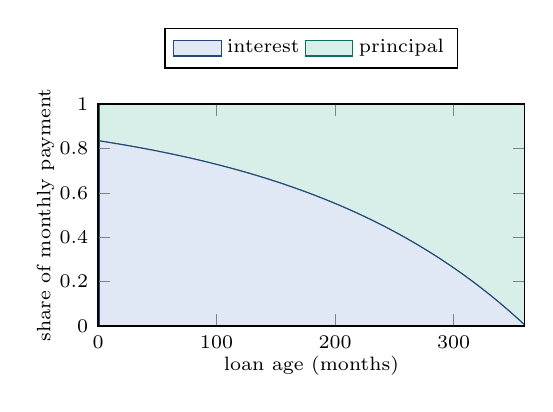
\begin{tikzpicture}
\begin{axis}[width=7.0cm,height=4.4cm, xlabel={loan age (months)}, ylabel={share of monthly payment},
  xmin=0,xmax=360, ymin=0, ymax=1, tick label style={font=\scriptsize},
  every axis x label/.style={at={(axis description cs:0.5,-0.09)},anchor=north,font=\scriptsize},
  every axis y label/.style={at={(axis description cs:-0.08,0.5)},rotate=90,anchor=south,font=\scriptsize},
  domain=1:360, samples=120, stack plots=y, area style,
  legend style={font=\scriptsize, at={(0.5,1.16)},anchor=south, legend columns=2}]
  \addplot[draw=accent, fill=nodeblue] {1-0.166*1.005^(x-1)} \closedcycle; \addlegendentry{interest}
  \addplot[draw=accent2, fill=nodeteal] {0.166*1.005^(x-1)} \closedcycle; \addlegendentry{principal}
\end{axis}
\end{tikzpicture}
\hspace{3mm}
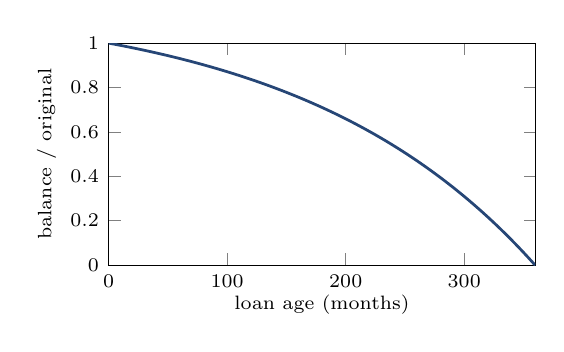
\begin{tikzpicture}
\begin{axis}[width=7.0cm,height=4.4cm, xlabel={loan age (months)}, ylabel={balance / original},
  xmin=0,xmax=360, ymin=0, ymax=1, tick label style={font=\scriptsize},
  every axis x label/.style={at={(axis description cs:0.5,-0.09)},anchor=north,font=\scriptsize},
  every axis y label/.style={at={(axis description cs:-0.1,0.5)},rotate=90,anchor=south,font=\scriptsize},
  domain=0:360, samples=120]
  \addplot[plotblue, line width=1pt] {(6.02-1.005^x)/5.02};
\end{axis}
\end{tikzpicture}
\caption{A 30-year fixed loan amortising (schematic). \textbf{Left:} the constant monthly
payment is mostly interest at first and mostly principal near the end; the crossover comes
surprisingly late (well past the half-way point in years). \textbf{Right:} the remaining
balance (UPB) therefore falls slowly at first and faster later. The model's \texttt{Loan Age},
\texttt{Current Actual UPB}, and \texttt{Remaining Months to Maturity} fields all track
positions along these curves.}
\end{figure}

\subsection{Fixed, adjustable, and the fine print}

Not all mortgages are the plain 30-year fixed loan above. The features that matter for our
data are:

\begin{itemize}[leftmargin=1.4em, itemsep=2pt]
  \item \textbf{FRM vs.\ ARM.} A \emph{fixed-rate mortgage} keeps one rate for life. An
        \emph{adjustable-rate mortgage} starts with a fixed period and then resets
        periodically to a market index. ARMs often begin with a low ``teaser'' rate that
        later jumps --- a common trigger for refinancing.
  \item \textbf{Interest-only} loans defer principal for a while; \textbf{prepayment
        penalties} charge the borrower for paying off early; \textbf{balloon} loans owe a
        lump sum at the end.
  \item \textbf{Conforming vs.\ jumbo.} Loans small enough and standard enough to be bought
        by the government-sponsored enterprises are ``conforming'' --- the Fannie Mae data is
        exactly this conforming population.
\end{itemize}

\begin{intuition}[Why the product type shows up in the model]
Each of these features bends borrower behaviour. An ARM about to reset, or a loan whose
prepayment penalty just expired, suddenly becomes far likelier to prepay --- which is why the
data carries \texttt{Amortization Type}, \texttt{Interest-Only Indicator}, and related fields,
and why the loan-age ``spikes'' in prepayment (Section~\ref{sec:features}) line up with reset
and penalty-expiry dates.
\end{intuition}

\subsection{How a mortgage ends: the two competing fates}

A mortgage can leave the books in two very different ways, and almost the entire dissertation
is about telling them apart.

\begin{itemize}[leftmargin=1.4em, itemsep=2pt]
  \item \textbf{Prepayment} --- the borrower pays the loan off \emph{early}, almost always by
        refinancing into a cheaper loan or selling the house. The lender gets their principal
        back, but loses the future interest they were counting on.
  \item \textbf{Default} --- the borrower stops paying. This unfolds through a
        \emph{delinquency ladder}: 30, then 60, then 90+ days past due, then
        \emph{foreclosure} (the legal seizure of the home), then \emph{REO} (``real-estate
        owned,'' the lender now holds and must sell the property).
\end{itemize}

Importantly, borrowers can \emph{cure} --- a loan 60 days late can return to current --- so the
ladder is climbed in both directions, not a one-way slide.

\begin{keyidea}[Competing risks]
Prepayment and default are \emph{competing risks}: a loan can only exit once, so the two
terminal outcomes compete for each loan. A model of mortgage behaviour must therefore predict
\emph{both} simultaneously rather than studying one in isolation --- which is precisely why the
seven-state transition model (Section~\ref{sec:states}) treats \texttt{prepaid},
\texttt{foreclosure}, and \texttt{REO} as distinct absorbing outcomes in one framework.
\end{keyidea}

\subsection{The borrower's two embedded options}

There is an elegant way to see why these two fates behave so differently. Holding a mortgage
is, for the borrower, like holding two financial \emph{options}.

\begin{itemize}[leftmargin=1.4em, itemsep=2pt]
  \item The \textbf{prepayment option} is a \emph{call} on the loan: the borrower may ``buy
        back'' their debt at par whenever they like. It pays to exercise when market rates fall
        below the loan's rate --- refinance, and capture the difference. This is the
        refinancing incentive.
  \item The \textbf{default option} is a \emph{put} on the house: the borrower may ``sell'' the
        property to the lender by handing over the keys. It is in the money when the home is
        worth less than the loan --- the borrower is \emph{underwater}.
\end{itemize}

\begin{intuition}[Why the option view matters --- and why it is not the whole story]
The option lens, developed in the classic mortgage literature (e.g.\ Schwartz \& Torous, 1989;
Deng, Quigley \& Van Order, 2000), says interest rates should drive prepayment and house
prices should drive default. That is broadly true and motivates which variables we feed the
model. But real borrowers do \emph{not} exercise these options with textbook precision: they
prepay late, default reluctantly, and respond to credit scores, loan size, and personal
circumstances in tangled, nonlinear ways. The gap between the clean option theory and messy
reality is exactly the territory a flexible deep-learning model is built to map.
\end{intuition}

\subsection{The risk drivers: how a loan is sized up}

A handful of standardised numbers summarise a loan's risk, and they recur as model features:

\begin{itemize}[leftmargin=1.4em, itemsep=2pt]
  \item \textbf{FICO} --- the borrower's credit score (roughly 300--850); higher means a
        stronger repayment history.
  \item \textbf{LTV / CLTV} --- \emph{loan-to-value} is the loan divided by the home's value;
        \emph{combined} LTV adds any second liens. High LTV means little equity cushion.
  \item \textbf{DTI} --- \emph{debt-to-income}, the share of the borrower's income consumed by
        debt payments; high DTI means a stretched borrower.
\end{itemize}

\begin{jargon}[Original vs.\ current LTV, and ``underwater'']
LTV at origination is fixed, but the one that drives behaviour is \emph{current} LTV: today's
balance over today's home value. As prices rise the borrower builds \emph{equity} (current LTV
falls) and can refinance easily; as prices fall they may go \emph{underwater} (current LTV above
100\%), unable to sell or refinance and likelier to default. Reconstructing current LTV from a
house-price index is one of the key feature-engineering steps in Section~\ref{sec:features}.
\end{jargon}

\subsection{The macro backdrop}

Borrowers do not act in a vacuum; a few economy-wide variables move everyone at once:

\begin{itemize}[leftmargin=1.4em, itemsep=2pt]
  \item \textbf{Interest rates.} The prevailing mortgage rate (we use the Freddie Mac PMMS
        series) sets the refinancing incentive. When it drops, prepayment surges.
  \item \textbf{House prices.} A house-price index (we use the FHFA HPI) updates each home's
        value and hence current LTV and equity, governing default pressure.
  \item \textbf{Unemployment.} Job loss is a classic trigger of delinquency; local
        unemployment is a standard default predictor.
\end{itemize}

\begin{intuition}[Common factors create correlation]
Because every loan in a region shares the same rates, prices, and unemployment, their fates are
\emph{correlated}: when rates fall, a whole pool tends to prepay together. This shared exposure
is what makes pool-level prediction (Section~\ref{sec:pool}) more than a trivial sum --- and, as
we will see, it is also why a mis-specified linear model's errors reinforce rather than cancel.
\end{intuition}

\subsection{Why prepayment is the hard one: seasoning and burnout}

\begin{jargon}[Seasoning and burnout]
\emph{Seasoning} is the tendency of prepayment to ramp up over a loan's first few years rather
than starting at full speed --- new borrowers rarely refinance immediately. \emph{Burnout} is
the opposite-end effect: after a refinancing wave, the borrowers left in a pool are the ones who
\emph{didn't} act, so the pool prepays less even when incentives return. Both are
\emph{path-dependent} --- they depend on the history a loan has lived through, not just today's
numbers.
\end{jargon}

These effects, layered on top of the already S-shaped response to incentive, make prepayment the
most violently nonlinear of all the transitions --- and the place where the deep model most
outperforms the linear one, at both the loan and pool level.

\subsection{Securitisation and mortgage-backed securities}

Finally, the reason any of this is worth millions of dollars: most of these loans are not held
by their originators but \emph{securitised}.

\begin{jargon}[Securitisation, pass-through, agency MBS, GSE]
\emph{Securitisation} bundles many loans into a pool and sells investors claims on the pool's
combined cash flows. The simplest claim is a \emph{pass-through}: borrowers' monthly principal
and interest flow through to investors pro rata. When the pool is guaranteed by a
\emph{government-sponsored enterprise} (GSE) such as Fannie Mae, the result is an \emph{agency
mortgage-backed security} (MBS). The GSE guarantee removes most \emph{credit} risk for the
investor --- but, crucially, \emph{not prepayment risk}.
\end{jargon}

\begin{figure}[H]
\centering
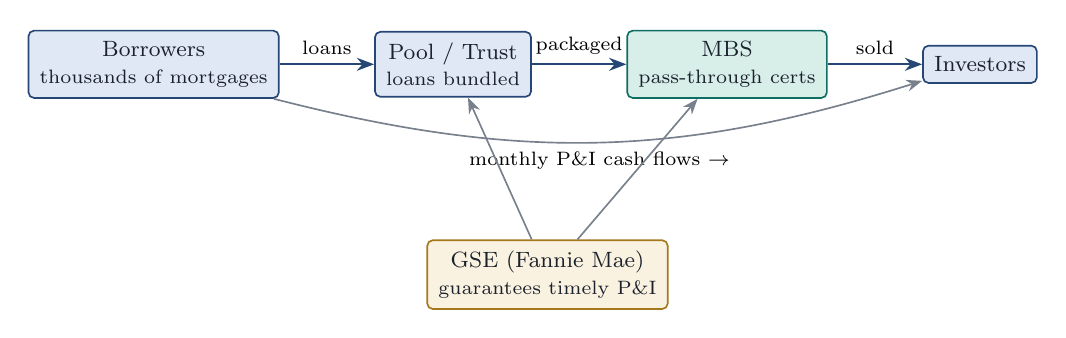
\begin{tikzpicture}[node distance=7mm and 12mm]
  \node[box, align=center] (bor) {Borrowers\\\scriptsize thousands of mortgages};
  \node[box, right=of bor] (pool) {Pool / Trust\\\scriptsize loans bundled};
  \node[tbox, right=of pool] (mbs) {MBS\\\scriptsize pass-through certs};
  \node[box, right=of mbs] (inv) {Investors};
  \node[abox, below=18mm of pool, xshift=12mm] (gse) {GSE (Fannie Mae)\\\scriptsize guarantees timely P\&I};
  \draw[flow] (bor)--(pool) node[midway,above,font=\scriptsize]{loans};
  \draw[flow] (pool)--(mbs) node[midway,above,font=\scriptsize]{packaged};
  \draw[flow] (mbs)--(inv) node[midway,above,font=\scriptsize]{sold};
  \draw[flow2] (bor) to[bend right=16] node[midway,below,font=\scriptsize]{monthly P\&I cash flows $\rightarrow$} (inv);
  \draw[flow2] (gse) -- (mbs);
  \draw[flow2] (gse) -- (pool);
\end{tikzpicture}
\caption{The securitisation chain. Loans are pooled and sold to investors as pass-through MBS;
borrowers' monthly principal and interest flow up to those investors. The GSE guarantee makes
the credit risk the investor's least worry --- leaving \emph{prepayment} as the dominant risk
they must forecast, which is what makes accurate pool-level prepayment prediction so valuable.}
\end{figure}

\begin{intuition}[Prepayment risk and ``negative convexity'']
An MBS investor is, in effect, \emph{short} the borrowers' prepayment option. When rates fall,
exactly when the investor would most like to keep their high-yielding bond, borrowers refinance
and hand the principal back early --- to be reinvested at the new, lower rate. When rates rise,
prepayments slow and the investor is stuck holding a below-market bond for longer. Heads the
investor loses a little, tails they lose a little: this asymmetry is called \emph{negative
convexity}, and it is why mispricing pool-level prepayment translates directly into mispriced
MBS.
\end{intuition}

\subsection{How the primer maps onto the model}

\begin{keyidea}[The whole primer, in one correspondence]
The mortgage's possible fates become the model's \textbf{seven states}; the risk drivers and
macro variables become its \textbf{features}; the embedded-option intuition tells us
\emph{which} features matter for \emph{which} transition; and the securitised pool is the
\textbf{pool-level target} whose prepayment the model must forecast. Everything in this primer
is, in the end, either a label, a feature, or the thing we are ultimately trying to price.
\end{keyidea}

% ======================================================================
\section{The raw material: the Fannie Mae loan tape}
\label{sec:data}

\subsection{What the data physically is}

The Fannie Mae Single-Family Loan Performance (SFLP) dataset is a \emph{loan-month
panel}. Read that phrase carefully, because it shapes everything.

\begin{jargon}[Loan-month panel]
A ``panel'' tracks many subjects over time. Here each \emph{subject} is one mortgage, and
we observe it \emph{every month} it is alive. So the unit of a single row is not ``a
loan'' but ``a loan in a particular month'' --- a \emph{loan-month}. One thirty-year
mortgage that survives to maturity contributes up to 360 rows, one per monthly report.
\end{jargon}

Concretely, the raw data we hold is:

\begin{itemize}[leftmargin=1.4em, itemsep=2pt]
  \item about \textbf{219 GB} spread over 26 quarterly CSV files (the largest single file
        is roughly 25 GB);
  \item \textbf{pipe-delimited} (\texttt{|} between fields) with \textbf{no header row} ---
        column identity is purely \emph{positional}, so the order of the 113 fields
        \emph{is} the contract;
  \item \textbf{113 fields} per row, with dates encoded as \texttt{MMYYYY}
        (e.g.\ \texttt{112013} means November 2013);
  \item partial and a little dirty: several quarters are missing, and at least three
        files are truncated downloads (one ``quarter'' contains only 15 distinct loans).
\end{itemize}

\begin{intuition}[Why the size is a real obstacle, not a footnote]
A 25 GB file will not fit in a laptop's memory, and the naive \texttt{pandas.read\_csv}
on it will crash the machine. The full panel is on the order of one to two \emph{billion}
loan-months. So a surprising amount of the dissertation's engineering effort goes into
\emph{never loading the whole thing at once}. That constraint --- not the statistics ---
is what dictates the architecture of the pipeline in Section~\ref{sec:pipeline}.
\end{intuition}

It helps to see our raw material beside the paper's, since the replication's credibility rests
on the data being comparable in spirit even though the source differs.

\begin{table}[H]
\centering
\caption{The two datasets at a glance. Ours is public and conforming; the paper's was
proprietary and spanned subprime as well as prime. The methodology transfers; the population
and provenance differ.}
\vspace{2pt}
\small
\begin{tabular}{>{\raggedright\arraybackslash}p{4.6cm} >{\raggedright\arraybackslash}p{4.8cm} >{\raggedright\arraybackslash}p{4.8cm}}
\toprule
 & \textbf{This dissertation} & \textbf{Original paper} \\
\midrule
Source & Fannie Mae SFLP (public) & CoreLogic (proprietary) \\
Population & prime, conforming & prime \emph{and} subprime \\
Scale & $\sim$1--2 billion loan-months; 219\,GB raw, 113 fields & $\sim$3.5 billion loan-months; $\sim$118 million mortgages \\
Span & $\sim$2000--2025 (includes COVID) & 1995--2014 \\
Macro covariates (first pass) & rate (PMMS) + price (FHFA HPI); fuller macro deferred & rich macro incl.\ zip-level prices, unemployment \\
Target & seven-state monthly transition & seven-state monthly transition \\
\bottomrule
\end{tabular}
\end{table}

\subsection{The fields that matter}

Of the 113 columns, most are post-default servicing and expense fields we will not use as
predictors. The ones that carry the modelling signal fall into a few families:

\begin{itemize}[leftmargin=1.4em, itemsep=2pt]
  \item \textbf{Identity and time:} \texttt{Loan Identifier} (stable across a loan's
        months --- this is the key that lets us follow a loan), and
        \texttt{Monthly Reporting Period} (the time index).
  \item \textbf{Origination characteristics} (fixed at the start): original interest rate,
        original balance (UPB), original term, original loan-to-value (LTV) and combined
        LTV, debt-to-income (DTI), borrower and co-borrower FICO credit scores, loan
        purpose, property type, occupancy, state, MSA, 3-digit zip.
  \item \textbf{Contemporary state} (changes month to month): current interest rate,
        current actual balance, loan age, remaining months to maturity, and the two fields
        that drive our target --- \texttt{Current Loan Delinquency Status} and
        \texttt{Zero Balance Code}.
\end{itemize}

\begin{jargon}[UPB]
\emph{Unpaid Principal Balance} --- how much of the loan the borrower still owes. The
\emph{current actual} UPB falling faster than the scheduled amortisation is a signal of
partial prepayment (``curtailment''); the UPB going to zero is the loan terminating.
\end{jargon}

% ======================================================================
\section{From a loan's life to a prediction problem}
\label{sec:states}

\subsection{The seven states}

We follow the paper in collapsing a mortgage's status into one of \textbf{seven states}:

\begin{center}
\texttt{current} $\to$ \texttt{30 dpd} $\to$ \texttt{60 dpd} $\to$ \texttt{90+ dpd}
$\to$ \texttt{foreclosure} $\to$ \texttt{REO} \quad and \quad \texttt{prepaid}
\end{center}

where ``dpd'' is days-past-due. A loan does \emph{not} march down this line in order: it
hops around. A borrower can miss a payment (\texttt{current} $\to$ \texttt{30 dpd}),
catch up the next month (\texttt{30 dpd} $\to$ \texttt{current}), and pay the loan off
years later (\texttt{current} $\to$ \texttt{prepaid}).

\begin{figure}[H]
\centering
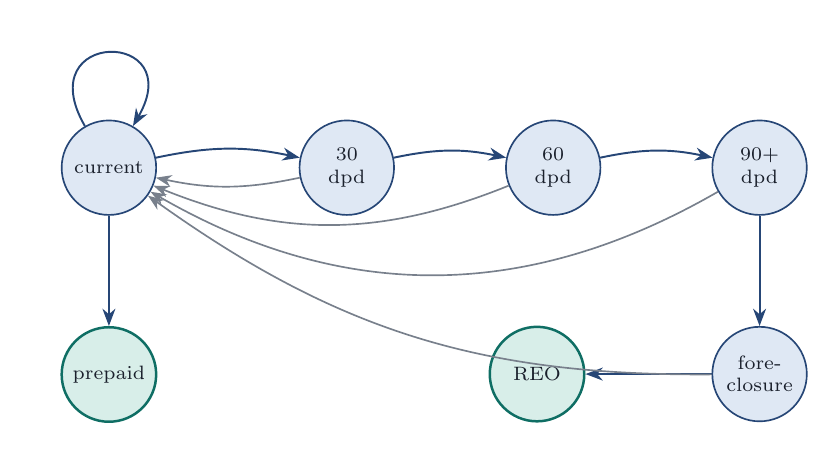
\begin{tikzpicture}[node distance=15mm]
  \node[st] (cur) {current};
  \node[st, right=18mm of cur] (d30) {30\\dpd};
  \node[st, right=14mm of d30] (d60) {60\\dpd};
  \node[st, right=14mm of d60] (d90) {90+\\dpd};
  \node[st, below=14mm of d90] (fc) {fore-\\closure};
  \node[abs, left=16mm of fc] (reo) {REO};
  \node[abs, below=14mm of cur] (pp) {prepaid};
  \draw[flow] (cur) to[bend left=12] (d30);
  \draw[flow] (d30) to[bend left=12] (d60);
  \draw[flow] (d60) to[bend left=12] (d90);
  \draw[flow2] (d30) to[bend left=12] (cur);
  \draw[flow2] (d60) to[bend left=22] (cur);
  \draw[flow2] (d90) to[bend left=30] (cur);
  \draw[flow] (cur) to[out=120,in=60,looseness=6] (cur);
  \draw[flow] (d90) -- (fc);
  \draw[flow] (fc) -- (reo);
  \draw[flow] (cur) -- (pp);
  \draw[flow2] (fc) to[bend left=18] (cur);
\end{tikzpicture}
\caption{The seven-state machine. Blue arrows are ``getting worse'' transitions, grey
arrows are ``curing'' back toward \texttt{current}, and the self-loop is staying current.
The two teal nodes, \texttt{prepaid} and \texttt{REO}, are \emph{absorbing}: once entered,
the loan leaves the sample. Note that \texttt{current} can jump straight to \texttt{prepaid}
(a refinance or sale) without passing through delinquency.}
\end{figure}

\begin{jargon}[REO and prepaid]
\texttt{REO} is ``real-estate owned'' --- the lender has taken the property after
foreclosure. \texttt{prepaid} means the loan ended early by being paid in full (usually a
refinance or a home sale). \texttt{REO} and \texttt{prepaid} are treated as
\emph{absorbing}: once a loan reaches them it leaves the sample, because there is nothing
more to predict.
\end{jargon}

\subsection{Where the seven states come from in the raw data}

The data does not hand us a tidy ``state'' column; we derive it from two fields.

\begin{itemize}[leftmargin=1.4em, itemsep=2pt]
  \item \texttt{Current Loan Delinquency Status} (a string \texttt{00},\,\texttt{01},
        \texttt{02},\,\texttt{03},\,\dots): \texttt{00} is current, \texttt{01} is 30 days
        late, \texttt{02} is 60, \texttt{03}\,+ is 90+ days late.
  \item \texttt{Zero Balance Code}: this is \emph{blank for every month except the loan's
        final, terminating month}. When present it tells us \emph{how} the loan ended ---
        code \texttt{01} = prepaid/matured, \texttt{09} = REO/deed-in-lieu, and a cluster
        of codes (\texttt{02},\,\texttt{03},\,\texttt{15},\,\texttt{97}) that map to a
        credit-event \texttt{foreclosure}.
\end{itemize}

So the rule, per loan-month, is: \emph{if a Zero Balance Code is present, the state is the
terminal state it encodes; otherwise the delinquency status governs.}

\begin{keyidea}[The supervised label is a transition, not a state]
For each loan-month we record the current state $U_t$ \emph{and} the same loan's state the
following month, $U_{t+1}$ (we call it \texttt{state\_next}, obtained with a window
function that looks one month ahead within each loan). The pair $(U_t, U_{t+1})$ is what
the model learns to predict. The label is the \emph{next} state given the current one and
everything we know today.
\end{keyidea}

\begin{figure}[H]
\centering
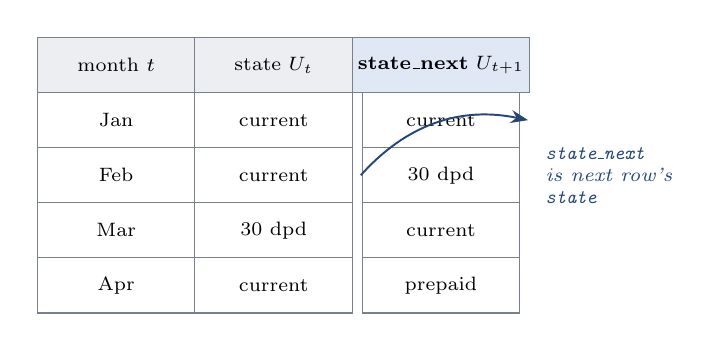
\begin{tikzpicture}[node distance=0mm]
  \matrix (m) [matrix of nodes, nodes={draw=derfr, minimum width=20mm, minimum height=7mm,
      font=\scriptsize, anchor=center, inner sep=2pt}, row sep=-\pgflinewidth, column sep=-\pgflinewidth]{
    |[fill=nodegray]| month $t$ & |[fill=nodegray]| state $U_t$ & |[fill=nodeblue]| \textbf{state\_next} $U_{t+1}$ \\
    Jan & current & current \\
    Feb & current & 30 dpd \\
    Mar & 30 dpd & current \\
    Apr & current & prepaid \\
  };
  \draw[flow, draw=accent] ($(m-3-2.east)+(1mm,0)$) to[bend left=30] ($(m-2-3.east)+(1mm,0)$);
  \node[font=\scriptsize\itshape, text=accent, align=left, right=2mm of m-3-3] {\texttt{state\_next}\\is next row's\\\texttt{state}};
\end{tikzpicture}
\caption{One loan's panel rows. The label \texttt{state\_next} for each month is simply that
same loan's \texttt{state} in the \emph{following} month --- a one-row shift. Because this
peeks one month into the future, the leakage-safe time mask in
Section~\ref{sec:pipeline} must be strict. The last row of an alive-but-current loan would
have an empty \texttt{state\_next}: that is the \emph{censored} case.}
\end{figure}

\begin{intuition}[Censoring: the loans that simply ``run out'']
Some loans are still alive and current on the last date in our data. They have no
\texttt{state\_next} --- not because anything happened, but because the data stops. These
are \emph{right-censored}, and we flag them. It would be a mistake to treat ``no
observed next month'' as ``the loan disappeared.'' Keeping a \texttt{censored} flag lets
the training code handle them correctly instead of inventing a fake terminal event.
\end{intuition}

\subsection{The empirical transition matrix --- our humble benchmark}

Before any neural network, there is an almost embarrassingly simple model we must beat.
Count, across the whole dataset, how often a loan in state $u$ moved to state $v$ next
month, and divide by how often it was in state $u$ at all:
\[
  \widehat{\Prob}_{\text{emp}}(v \mid u)
  \;=\; \frac{\#\{\text{loan-months: } u \to v\}}{\#\{\text{loan-months in } u\}}.
\]
Stack these into a $7\times 7$ matrix and you have the \emph{empirical transition
matrix}. It predicts the next state using \emph{only} the current state --- it ignores
FICO, rates, balance, everything.

Its quality as a model is measured by the same loss we will use for the networks --- the
negative log-likelihood it assigns to the realised transitions:
\begin{equation}
  \text{loss}_{\text{emp}}
  \;=\; -\frac{1}{M}\sum_{(u\to v)\ \text{observed}}
        \log \widehat{\Prob}_{\text{emp}}(v \mid u),
  \label{eq:emploss}
\end{equation}
where $M$ is the number of transitions. Every richer model must drive this number down.

\begin{intuition}[Why bother with a benchmark this dumb?]
Because a model that cannot beat ``just use the historical frequencies'' has learned
nothing useful from all those covariates. The empirical matrix sets the bar. We will
measure every model --- logistic regression, shallow net, deep net --- by how far below
this benchmark's loss they can push (Section~\ref{sec:training}). Most of the
mass sits on \texttt{current}~$\to$~\texttt{current}, so a good model must earn its keep
on the rare, costly transitions: into delinquency, foreclosure, and prepayment.
\end{intuition}

\begin{intuition}[How lopsided the classes really are]
``Most of the mass'' undersells it. In a healthy prime book the overwhelming majority of
loan-months are \texttt{current}~$\to$~\texttt{current}, while the credit-event transitions
(into foreclosure and REO) are well under 1\% of rows --- the events that matter most for
cashflows are the rarest in the data. This is why the pipeline samples in a
\emph{stratified} way: it keeps every scarce foreclosure and REO transition and down-samples
the torrent of \texttt{current}~$\to$~\texttt{current}, then corrects for that thinning with
the importance weights of Section~\ref{sec:training}. After thinning, the training export is
on the order of tens of millions of rows ($\sim$74 M) over roughly thirty features --- small
enough to train on, balanced enough to learn the rare events. The imbalance is not a nuisance
to be smoothed away; it is the reason the rare-transition accuracy in the results tables is
the number to watch.
\end{intuition}

% ======================================================================
\section{The data pipeline: turning 219 GB into something trainable}
\label{sec:pipeline}

This section is the engineering heart of the project. It earns its length because if the
pipeline is wrong --- if it leaks the future, double-counts a loan, or silently mixes a
truncated file into training --- then every clever thing downstream is built on sand.

\subsection{The one rule that drives the whole design}

\begin{keyidea}[Never load a full quarter into memory]
Every stage operates on \emph{bounded chunks} --- a row-group, a batch, one quarter ---
or pushes the heavy lifting down into a database engine that streams from disk. No stage
ever calls a full \texttt{.collect()} on the whole panel.
\end{keyidea}

The stack chosen to honour that rule is \textbf{Parquet + DuckDB + Polars}:

\begin{itemize}[leftmargin=1.4em, itemsep=2pt]
  \item \textbf{Parquet} (with \texttt{zstd} compression) is a \emph{columnar} file
        format. Storing by column means a query that needs 6 of 113 columns reads about
        5\% of the bytes, and the dataset compresses roughly 4--8$\times$ --- the 219 GB
        raw lands in $\sim$30--50 GB.
  \item \textbf{DuckDB} runs SQL \emph{directly over} the Parquet files, reading only the
        columns and rows a query touches and spilling to disk when memory is tight. You
        can \texttt{SELECT \dots\ WHERE acq\_quarter='2020Q4'} without loading anything
        else.
  \item \textbf{Polars} is a DataFrame library whose \emph{lazy} \texttt{scan}/\texttt{sink}
        operations stream through data in bounded memory and parallelise across cores.
\end{itemize}

\begin{jargon}[Columnar vs row storage]
A spreadsheet stores row by row: all of Alice's fields, then all of Bob's. Columnar
storage keeps all the FICO scores together, all the balances together, and so on. If you
only want FICO and balance, columnar lets you read just those two stripes off disk and
skip the other 111 fields entirely. For analytics over a few columns of a huge table,
this is the difference between minutes and hours.
\end{jargon}

\subsection{The six stages}

The pipeline is six \emph{idempotent}, \emph{per-quarter} stages --- re-running skips work
already done, so a crash mid-run is recoverable.

\begin{enumerate}[leftmargin=1.6em, itemsep=4pt]
  \item \textbf{Inventory \& integrity audit.} Before trusting anything, catalogue every
        file: row count, distinct loans, time span, field count. Quarantine the truncated
        files. \emph{This is non-negotiable and goes first} --- you do not model against
        a dataset whose coverage you have not mapped.
  \item \textbf{Stream CSV $\to$ Parquet.} Convert each raw CSV to compressed Parquet in
        bounded chunks, keeping a faithful string-typed copy (so this stage never fails on
        a dirty value).
  \item \textbf{Clean \& standardise.} Cast types (\texttt{MMYYYY}~$\to$~date,
        floats~$\to$~32-bit, sentinels like FICO \texttt{9999}~$\to$~null), project down
        to the columns the model needs, and add calendar keys (\texttt{period\_ym},
        \texttt{orig\_ym}) and \emph{missingness indicators}.
  \item \textbf{Build the transition panel.} Derive \texttt{state}, \texttt{state\_next}
        and \texttt{censored} with a per-loan ordered window, plus a \texttt{shard} key
        (see below).
  \item \textbf{Views \& stratified sampling.} Expose the panel through DuckDB and draw
        RAM-sized samples that \emph{keep all the rare transitions} (foreclosure, REO) and
        down-sample the overwhelming \texttt{current}~$\to$~\texttt{current} mass.
  \item \textbf{QA \& reconciliation.} Prove each stage preserved row counts, audit null
        rates, print the $7\times 7$ transition counts, and confirm no duplicate
        loan-months.
\end{enumerate}

\begin{figure}[H]
\centering
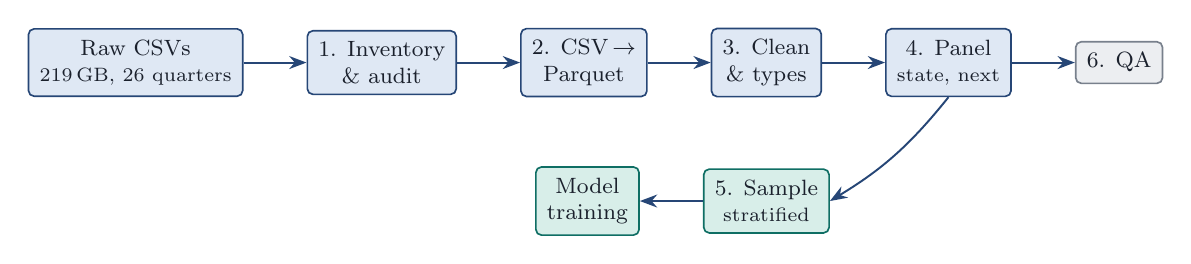
\begin{tikzpicture}[node distance=5mm and 8mm]
  \node[box] (raw) {Raw CSVs\\{\scriptsize 219\,GB, 26 quarters}};
  \node[box, right=of raw] (inv) {1. Inventory\\\& audit};
  \node[box, right=of inv] (pq) {2. CSV\,$\to$\\Parquet};
  \node[box, right=of pq] (cl) {3. Clean\\\& types};
  \node[box, right=of cl] (pan) {4. Panel\\{\scriptsize state, next}};
  \node[tbox, below=9mm of cl] (samp) {5. Sample\\{\scriptsize stratified}};
  \node[tbox, left=of samp] (mod) {Model\\training};
  \node[gbox, right=8mm of pan] (qa) {6. QA};
  \draw[flow] (raw)--(inv); \draw[flow] (inv)--(pq); \draw[flow] (pq)--(cl);
  \draw[flow] (cl)--(pan); \draw[flow] (pan)--(qa);
  \draw[flow] (pan.south) to[bend left=10] (samp.east);
  \draw[flow] (samp)--(mod);
\end{tikzpicture}
\caption{The six-stage pipeline. Raw immutable CSVs flow left to right into a compressed,
queryable Parquet lake; Stage~5 draws RAM-sized stratified samples for the model. The
governing constraint is that no arrow ever requires a full quarter in memory --- everything
streams in bounded chunks.}
\end{figure}

\subsection{Two subtle correctness rules}

Two rules deserve to be singled out because they are easy to get wrong and catastrophic
when you do.

\begin{intuition}[Rule 1: the leakage-safe time mask]
Our label looks \emph{one month into the future} (\texttt{state\_next}). So if we want to
train ``on everything up to month $T$,'' we must filter on \texttt{period\_ym}~$<T$,
\emph{strictly}, not~$\le T$. Including month $T$ itself would feed the model a label
($T{+}1$'s state) that lies past the cutoff --- the future leaking into the past. A
one-character slip ($<$ vs $\le$) silently inflates every backtest. This is the kind of
bug that makes a model look brilliant and then fail in production.
\end{intuition}

\begin{intuition}[Rule 2: shard by loan, never split a loan across train and test]
We bucket each loan into one of $N$ shards via a deterministic hash of its
\texttt{Loan Identifier}: \texttt{shard = hash(loan\_id) \% N\_SHARDS}. Because the hash
is keyed on the loan, \emph{every month of a given loan lands in the same shard.} That
guarantees a loan never straddles train and test --- which would let the model peek at
the same borrower's other months --- and it gives us a cheap, reproducible way to stream
random minibatches: shuffle shard order, load one shard (RAM-sized), shuffle within it,
yield batches. (This is exactly the hash-table-to-folders trick the original paper
describes for de-biasing minibatches.)
\end{intuition}

\begin{derivation}[Why the empirical transition matrix needs the panel to be exactly right]
The benchmark counts $u\to v$ transitions. If a single loan's months were accidentally
split across two shards, or a truncated file's loans leaked in, those counts --- and
therefore the benchmark, and therefore every comparison against it --- would be quietly
wrong. The unglamorous QA stage is what lets you trust the headline numbers later.
\end{derivation}

% ======================================================================
\section{Feature engineering: the economics in the inputs}
\label{sec:features}

Raw fields are not yet good predictors. The paper's most important findings live in a few
\emph{engineered} features that encode mortgage economics. Three are worth understanding
deeply, because they are where the nonlinearities the whole project is about actually
appear.

\subsection{The refinancing incentive (and why it is so nonlinear)}

A borrower refinances --- i.e.\ prepays the old loan --- when the market rate has fallen
enough below their loan's rate to make it worthwhile. So the natural feature is the
\emph{rate incentive}:
\[
  \text{incentive}_t \;=\; (\text{the loan's note rate}) \;-\; (\text{current market mortgage rate}).
\]
For the market rate we use the Freddie Mac \textbf{PMMS} (Primary Mortgage Market Survey),
a long weekly series of the prevailing 30-year rate.

\begin{jargon}[PMMS]
Freddie Mac's Primary Mortgage Market Survey: the standard published series for ``the
mortgage rate this week.'' It is the yardstick against which a borrower's own rate is
high or low. Note the small irony of our project: the \emph{loans} come from Fannie Mae,
but the \emph{rate series} comes from Freddie Mac --- they are independent public sources.
\end{jargon}

\begin{intuition}[The incentive curve is an S, not a line]
You might guess prepayment rises smoothly with incentive. It does not. When incentive is
negative (your rate is below market) almost nobody refinances --- flat. As incentive
turns positive there is a steep surge --- people pounce on the savings. Then it
\emph{plateaus}: past a point, everyone who was going to refinance already has. The
sensitivity of prepayment to incentive therefore changes in \emph{both magnitude and
sign} along the curve. A linear model, which assumes a single constant slope, is
structurally incapable of fitting this --- and prepayment is where the paper finds the
strongest nonlinearities of all. This single picture is the moral motivation for using a
neural network.
\end{intuition}

\begin{figure}[H]
\centering
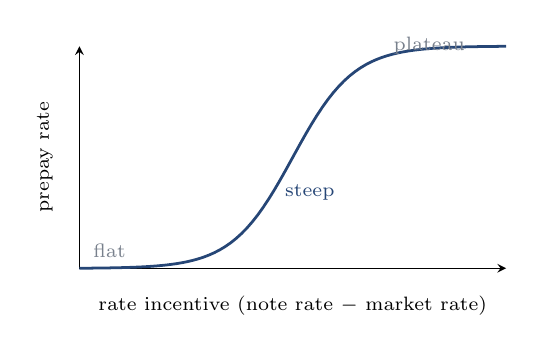
\begin{tikzpicture}
\begin{axis}[width=7.0cm, height=4.4cm, xlabel={rate incentive (note rate $-$ market rate)},
  ylabel={prepay rate}, xtick=\empty, ytick=\empty, axis lines=left,
  every axis x label/.style={at={(axis description cs:0.5,-0.08)},anchor=north,font=\scriptsize},
  every axis y label/.style={at={(axis description cs:-0.04,0.5)},rotate=90,anchor=south,font=\scriptsize},
  domain=-4:6, samples=80, clip=false]
  \addplot[plotblue, line width=1pt] {0.06+0.5/(1+exp(-1.4*(x-1)))};
  \node[font=\scriptsize,text=derfr,anchor=west] at (axis cs:-3.9,0.10) {flat};
  \node[font=\scriptsize,text=plotblue,anchor=north] at (axis cs:1.4,0.27) {steep};
  \node[font=\scriptsize,text=derfr,anchor=south] at (axis cs:4.2,0.52) {plateau};
\end{axis}
\end{tikzpicture}
\hspace{3mm}
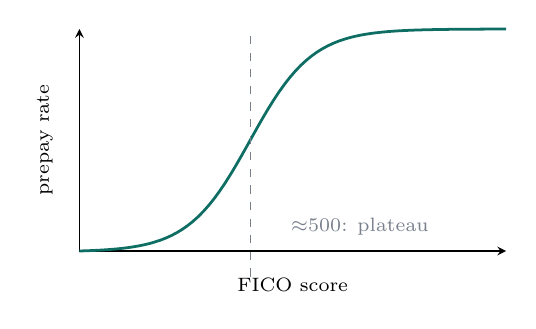
\begin{tikzpicture}
\begin{axis}[width=7.0cm, height=4.4cm, xlabel={FICO score}, ylabel={prepay rate},
  xtick=\empty, ytick=\empty, axis lines=left,
  every axis x label/.style={at={(axis description cs:0.5,-0.08)},anchor=north,font=\scriptsize},
  every axis y label/.style={at={(axis description cs:-0.04,0.5)},rotate=90,anchor=south,font=\scriptsize},
  domain=300:850, samples=80, clip=false]
  \addplot[plotteal, line width=1pt] {0.05+0.45/(1+exp(-0.025*(x-520)))};
  \draw[derfr,dashed] (axis cs:520,0) -- (axis cs:520,0.5);
  \node[font=\scriptsize,text=derfr,anchor=west] at (axis cs:560,0.10) {$\approx$500: plateau};
\end{axis}
\end{tikzpicture}
\caption{Two of the strong nonlinearities a linear model cannot capture (schematic, after the
paper's empirical figures). \textbf{Left:} prepayment versus refinancing incentive is
S-shaped --- flat, then a steep surge, then a plateau. \textbf{Right:} prepayment rises with
FICO but levels off above roughly 500. A single slope cannot describe either curve.}
\end{figure}

\begin{jargon}[Burnout]
A pool that has already lived through a refinancing wave is left with the borrowers who
\emph{didn't} refinance --- the sluggish, the credit-impaired, the inattentive. So even
at the same incentive, a ``burned-out'' pool prepays less. Burnout is a path-dependent
feature: it depends on the history of incentives the loan has seen, not just today's.
\end{jargon}

\subsection{Current LTV (using a house-price index)}

Original LTV is fixed at origination, but what matters for default and refinancing is the
\emph{current} loan-to-value: today's balance over today's home value. We do not observe
each home's price monthly, so we update it with the FHFA House Price Index (HPI):
\[
  \text{current LTV}_t \;\approx\;
  \frac{\text{current UPB}_t}{\text{original value}\times \dfrac{\text{HPI}_t}{\text{HPI}_{\text{orig}}}}.
\]

\begin{jargon}[FHFA HPI]
The Federal Housing Finance Agency's House Price Index measures how home prices have moved
over time, available at national, state, and metro levels. Multiplying the original home
value by the ratio of current-to-origination HPI gives an estimate of today's value
without an appraisal.
\end{jargon}

\begin{intuition}[Why current LTV drives both default and prepayment]
A borrower deep underwater (current LTV well above 100\%) can neither sell at a profit nor
easily refinance, and is likelier to default --- the ``put option'' on the house is in
the money. A borrower with lots of equity (low current LTV) refinances easily. So the same
variable pulls two different transitions, which is part of why the paper models all
transitions with \emph{one} shared network rather than separate models.
\end{intuition}

\subsection{Path-dependent delinquency counts (a recommendation)}

The paper finds something striking: for predicting \texttt{current}~$\to$~\texttt{30 dpd},
the dominant variable is not FICO or LTV but \emph{the number of times the borrower was 30
days late in the past 12 months}. Recent behaviour predicts near-future behaviour far
better than static credit characteristics.

\begin{keyidea}[Engineer the rolling delinquency counts]
Our current schema does not yet build these path-dependent counts (number of times 30/60/90+
days late in the trailing 12 months; number of times current). The paper's results say
they are among the most important predictors for the delinquency transitions. Adding them
is one of the highest-value feature-engineering steps available to the replication.
\end{keyidea}

\subsection{Which features actually matter (evidence from the paper)}

This is not just intuition --- the paper measures it. For each transition it computes the
\emph{average absolute gradient} of the fitted network's output with respect to each input:
how much the predicted probability moves when that feature is nudged. The result for the
\state{current}~$\to$~\state{prepaid} transition (the paper's Table~12, five-layer network) is
worth reading closely, because almost every feature we engineered above appears near the top.

\begin{table}[H]
\centering
\caption{Top features by average absolute gradient for \state{current}~$\to$~\state{prepaid},
five-layer network (original paper, Table~12). Larger means the predicted prepayment
probability is more sensitive to that feature.}
\vspace{2pt}
\small
\begin{tabular}{>{\raggedright\arraybackslash}p{9.2cm} r}
\toprule
\textbf{Feature} & \textbf{Avg.\ $|\text{gradient}|$} \\
\midrule
Current outstanding balance & 0.1878 \\
Original loan balance & 0.0856 \\
Original interest rate & 0.0503 \\
Current rate $-$ national mortgage rate \;\textit{(the refinancing incentive)} & 0.0478 \\
Original rate $-$ national mortgage rate & 0.0463 \\
Zip-code house-price change since origination \;\textit{(drives current LTV)} & 0.0386 \\
Number of times 30 days delinquent in last 12 months \;\textit{(path-dependent)} & 0.0384 \\
Number of times 60 days delinquent in last 12 months \;\textit{(path-dependent)} & 0.0362 \\
Time since origination \;\textit{(seasoning)} & 0.0306 \\
FICO score & 0.0293 \\
State unemployment rate & 0.0214 \\
LTV ratio & 0.0116 \\
\bottomrule
\end{tabular}
\end{table}

\begin{intuition}[Reading the importance table --- it validates the whole section]
Every engineered quantity from this section earns its place. The \textbf{refinancing
incentive} (current rate minus the national rate) sits near the top; the \textbf{house-price
change} that drives current LTV is just below it; the \textbf{path-dependent delinquency
counts} we recommended building rank above FICO and far above the static LTV ratio; and
\textbf{seasoning} (time since origination) is material. Two lessons stand out. First,
\emph{balance} variables dominate prepayment --- larger loans have more dollars of interest to
save by refinancing, so they respond most. Second, the celebrated static credit
characteristics (FICO at 0.0293, LTV at 0.0116) are \emph{less} influential than the dynamic,
path-dependent, and macro-linked variables --- which is precisely why a model that can exploit
those richer features, nonlinearly, pulls so far ahead of a plain logistic regression.
\end{intuition}

\begin{intuition}[A different transition, a different king]
Importance is transition-specific. For \state{current}~$\to$~\state{30 dpd}, the paper reports
that the \emph{number of times the borrower was 30 days late in the past year} dominates all
other variables --- recent behaviour, not credit score, predicts the near-future slip into
delinquency. This is the empirical backing for engineering the rolling delinquency counts, and
a reminder that the single shared network has to serve very different importance rankings across
the seven destinations at once.
\end{intuition}

\subsection{The standardisation discipline}

Continuous inputs (rates, balances, ages, LTV, DTI, FICO) live on wildly different scales,
so we standardise them (subtract mean, divide by standard deviation). Heavily skewed
quantities like balance are log-transformed first. For a feature column $x_j$ with
training-set mean $\mu_j$ and standard deviation $\sigma_j$,
\begin{equation}
  \tilde{x}_j \;=\; \frac{x_j - \mu_j}{\sigma_j},
  \qquad\text{or for skewed columns}\qquad
  \tilde{x}_j \;=\; \frac{\log(1+x_j) - \mu_j^{\log}}{\sigma_j^{\log}} .
  \label{eq:standardize}
\end{equation}

\begin{intuition}[Why standardise at all, and why the log first]
Gradient descent struggles when one input ranges over $[300,850]$ (FICO) and another over
$[0,1]$ (a flag): the loss surface becomes a stretched ravine that the optimiser bounces
across slowly. Rescaling every feature to mean~0, variance~1 makes the surface rounder and
training faster and more stable. The log on balances pulls in a long right tail (a few
million-dollar loans among many small ones) so the post-transform values are roughly
symmetric rather than dominated by a handful of giants.
\end{intuition}

\begin{intuition}[Compute the scaler on the training slice only]
It is tempting to standardise the whole dataset once. That leaks: the mean and standard
deviation would be computed using future and test data the model is not supposed to have
seen. The rule is to fit the scaler on the \emph{training slice only}, for each backtest
window, and store it. Baking standardised values into the data lake would be wrong for
every rolling window and would quietly contaminate every result.
\end{intuition}

% ======================================================================
\section{The neural network, built from logistic regression up}
\label{sec:nn}

This is the modelling core. We build it in five moves, each a small step from the last, so
that by the end the deep network feels inevitable rather than magical. Throughout, $x$
denotes the vector of explanatory variables for one loan-month (the engineered features of
Section~\ref{sec:features}), and $\mathcal{U}=\{\state{current},\state{30dpd},\dots,
\state{prepaid}\}$ is the set of $K=7$ states.

\subsection{Move 0: what the model must output}

For a loan currently in some state, in month $t-1$, with features $x = X^n_{t-1}$, we want
the probability of being in each state $u$ next month:
\begin{equation}
  \Prob\!\left[U^n_t = u \mid \mathcal{F}_{t-1}\right] \;=\; h_\theta(u,\, x),
  \qquad u \in \mathcal{U},
  \label{eq:transition}
\end{equation}
where $\theta$ are parameters we will estimate. For this to be a valid probability
distribution, the seven numbers $h_\theta(u,x)$ must be non-negative and sum to one. The
collection of these conditional probabilities, for every starting state, \emph{is} the
conditional transition matrix --- the model's version of the empirical matrix from
Section~\ref{sec:states}, but now depending on $x$.

\begin{jargon}[$\mathcal{F}_{t-1}$, the information set]
$\mathcal{F}_{t-1}$ is shorthand for ``everything known up to month $t-1$.'' Equation
\eqref{eq:transition} says: given all we know today, here is the probability of each state
tomorrow. The model is \emph{conditional} on the present, which is what makes it useful
for forecasting.
\end{jargon}

\subsection{Move 1: the softmax turns numbers into probabilities}

Suppose a model produces seven real-valued ``scores'' $z = (z_1,\dots,z_K)$, one per state
--- these can be any real numbers, positive or negative. The \textbf{softmax} function
squashes them into a probability distribution:
\begin{equation}
  \softmax(z)_k \;=\; \frac{e^{z_k}}{\sum_{j=1}^{K} e^{z_j}},
  \qquad k = 1,\dots,K.
  \label{eq:softmax}
\end{equation}
Exponentiating makes every entry positive; dividing by the sum makes them add to one.

\begin{intuition}[Why exponentials?]
Softmax rewards bigger scores disproportionately --- a score that is 2 larger becomes
$e^2 \approx 7.4$ times more probable, not 2 more. This ``soft'' winner-take-most behaviour
is exactly right for classification: the state with the highest score gets most of the
probability mass, but the others keep a sliver. It is the smooth, differentiable cousin of
just picking the maximum, and differentiability is what lets us train by gradient descent.
\end{intuition}

\subsection{Move 2: logistic regression is softmax of a straight line}

The simplest model feeds a \emph{linear} function of the features into the softmax:
\begin{equation}
  h_\theta(u, x) \;=\; \softmax\!\left(W x + b\right)_u,
  \qquad W \in \R^{K \times d_X},\;\; b \in \R^{K}.
  \label{eq:logreg}
\end{equation}
This is \emph{multinomial logistic regression} --- the workhorse of the empirical mortgage
literature. Here $\theta = (W, b)$. It is the \textbf{zero-hidden-layer} network, and it
will be our linear straw man throughout.

\begin{intuition}[Its fatal limitation in one line]
The output $h_\theta(u,x)$ can only bend in the directions encoded by the rows of $W$ ---
it is a fixed linear function of $x$ passed through a fixed squashing. It cannot represent
the S-shaped incentive curve, the FICO plateau, or the way two variables \emph{interact}.
For prepayment, where those nonlinearities are strongest, it is structurally
mis-specified. Everything below is a way to relax exactly this limitation.
\end{intuition}

\subsection{Move 3: from fixed features to \emph{learned} features}

A standard fix is to first transform $x$ through some basis functions
$\phi(x) = (\phi_1(x),\dots,\phi_{d_\phi}(x))$ --- polynomials, splines, step functions ---
and run logistic regression on those:
\(
  h_\theta(u,x) = \softmax(W\phi(x) + b)_u .
\)
The catch: \emph{you have to choose $\phi$ in advance}, and if your guess is wrong, the
model fits poorly. With dozens of mortgage variables interacting in unknown ways, guessing
the right basis by hand is hopeless.

\begin{keyidea}[The neural-network idea]
Instead of fixing the feature functions $\phi$ ahead of time, \emph{learn them from the
data}. Replace $\phi$ with a \emph{parameterised} transformation $\phi_\theta$ whose
parameters are estimated alongside $W$ and $b$. A neural network is precisely a flexible,
trainable $\phi_\theta$ stacked under a final softmax.
\end{keyidea}

\subsection{Move 4: stacking layers}

A neural network builds $\phi_\theta$ by composing simple operations called \emph{layers}.
Each layer takes the previous layer's output, applies (i) a linear map, then (ii) a simple
element-wise nonlinearity $\sigma$. Writing $h_{\theta,0}(x) = x$ for the inputs, the
output of layer $\ell$ is
\begin{equation}
  h_{\theta,\ell}(x) \;=\; \sigma\!\left(W_\ell\T\, h_{\theta,\ell-1}(x) + b_\ell\right),
  \qquad \ell = 1,\dots,L-1,
  \label{eq:layer}
\end{equation}
with $W_\ell \in \R^{d_{\ell-1}\times d_\ell}$ and $b_\ell \in \R^{d_\ell}$. The final
layer applies the softmax instead of $\sigma$, producing the seven probabilities:
\begin{equation}
  h_\theta(u, x) \;=\; \softmax\!\left(W_L\T\, h_{\theta,L-1}(x) + b_L\right)_u .
  \label{eq:output}
\end{equation}
The full parameter vector is $\theta = (W_1,\dots,W_L,\, b_1,\dots,b_L)$. The layers
strictly between input and output are the \emph{hidden} layers; a network with $L-1$ hidden
layers and $L=1$ (no hidden layers) collapses back to logistic regression
\eqref{eq:logreg}. Each hidden layer's output becomes the ``learned basis functions'' for
the next.

\begin{jargon}[Hidden layer, unit, activation]
A \emph{hidden layer} is an intermediate stage of computation you never directly observe
--- its outputs are internal features the network invents. Each coordinate of a layer is a
\emph{unit} (or neuron): one affine combination of the previous layer followed by the
nonlinearity $\sigma$, called the \emph{activation function}. ``Depth'' is the number of
layers; ``width'' is the number of units per layer.
\end{jargon}

Zooming in on a single unit makes \eqref{eq:layer} concrete. Unit $k$ of layer $\ell$
computes one number from the whole previous layer:
\begin{equation}
  \bigl(h_{\theta,\ell}(x)\bigr)_k
  \;=\; \sigma\!\Bigl(\underbrace{\textstyle\sum_{j} (W_\ell)_{jk}\,\bigl(h_{\theta,\ell-1}(x)\bigr)_j + (b_\ell)_k}_{\text{a weighted vote of the previous layer}}\Bigr).
  \label{eq:unit}
\end{equation}
Each weight $(W_\ell)_{jk}$ says how strongly feature $j$ of the previous layer feeds unit
$k$; the bias shifts the threshold; the activation decides whether the unit ``fires.''

\subsection{The activation: ReLU}

The element-wise nonlinearity we use is the \textbf{rectified linear unit}:
\begin{equation}
  \sigma(x) \;=\; \relu(x) \;=\; \max(0,\, x).
  \label{eq:relu}
\end{equation}
It passes positive values through unchanged and zeroes out negatives. The paper found ReLU
gave both better accuracy and faster convergence than the classic sigmoid
$\sigma(x)=1/(1+e^{-x})$.

\begin{intuition}[Why a kink is enough]
ReLU looks almost laughably simple --- a hinge. But stacking many hinged units lets the
network assemble arbitrarily intricate piecewise-linear surfaces, the way many short
straight segments can trace any curve. The flat-zero region also makes gradients cheap and
stable to propagate, which matters when you are taking hundreds of millions of gradient
steps. Crucially, \emph{without} a nonlinearity, stacking linear layers would just give one
big linear map --- no expressive gain at all. The nonlinearity is what makes depth worth
having.
\end{intuition}

\subsection{Our concrete architecture}

Cross-validation in the paper selected \textbf{five hidden layers} of widths
\[
  200 \;\to\; 140 \;\to\; 140 \;\to\; 140 \;\to\; 140,
\]
each with ReLU, feeding a final softmax over the $K=7$ states. So a single loan-month's
feature vector $x$ flows:
\[
  x \in \R^{d_X}
  \;\xrightarrow{\;W_1,\,b_1,\,\relu\;}\; \R^{200}
  \;\xrightarrow{\;\relu\;}\; \R^{140}
  \;\xrightarrow{\;\relu\;}\; \R^{140}
  \;\xrightarrow{\;\relu\;}\; \R^{140}
  \;\xrightarrow{\;\relu\;}\; \R^{140}
  \;\xrightarrow{\;\softmax\;}\; \Delta^{6},
\]
where $\Delta^6$ is the set of probability distributions over the seven states.

\begin{figure}[H]
\centering
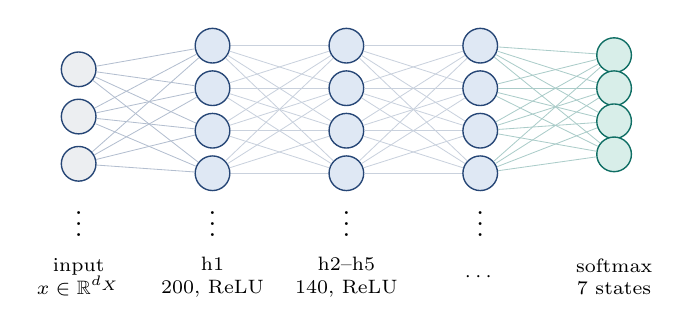
\begin{tikzpicture}[x=17mm, y=6mm]
  \def\lxin{0} \def\lxa{1} \def\lxb{2} \def\lxc{3} \def\lxd{4}
  \foreach \i in {1,2,3} \node[neuron, fill=nodegray] (in\i) at (\lxin, {2-\i}) {};
  \node at (\lxin,-2.1) {$\vdots$};
  \node[font=\scriptsize, align=center] at (\lxin,-3.4) {input\\$x\in\mathbb{R}^{d_X}$};
  \foreach \i in {1,...,4} \node[neuron] (h1\i) at (\lxa, {2.4-\i*0.9}) {};
  \node at (\lxa,-2.1) {$\vdots$};
  \node[font=\scriptsize, align=center] at (\lxa,-3.4) {h1\\200, ReLU};
  \foreach \i in {1,...,4} \node[neuron] (h2\i) at (\lxb, {2.4-\i*0.9}) {};
  \node at (\lxb,-2.1) {$\vdots$};
  \node[font=\scriptsize, align=center] at (\lxb,-3.4) {h2--h5\\140, ReLU};
  \foreach \i in {1,...,4} \node[neuron] (h3\i) at (\lxc, {2.4-\i*0.9}) {};
  \node at (\lxc,-2.1) {$\vdots$};
  \node[font=\scriptsize] at (\lxc,-3.4) {$\cdots$};
  \foreach \i in {1,...,4} \node[neuron, draw=accent2, fill=nodeteal] (o\i) at (\lxd, {2.0-\i*0.7}) {};
  \node[font=\scriptsize, align=center] at (\lxd,-3.4) {softmax\\7 states};
  \foreach \a in {1,2,3} \foreach \b in {1,...,4} \draw[draw=accent!35, line width=0.3pt] (in\a)--(h1\b);
  \foreach \a in {1,...,4} \foreach \b in {1,...,4} \draw[draw=accent!25, line width=0.3pt] (h1\a)--(h2\b);
  \foreach \a in {1,...,4} \foreach \b in {1,...,4} \draw[draw=accent!25, line width=0.3pt] (h2\a)--(h3\b);
  \foreach \a in {1,...,4} \foreach \b in {1,...,4} \draw[draw=accent2!35, line width=0.3pt] (h3\a)--(o\b);
\end{tikzpicture}
\caption{The architecture. The feature vector enters on the left; each hidden layer applies
a linear map then a ReLU (equations~\eqref{eq:layer}, \eqref{eq:relu}); the final teal layer
applies the softmax \eqref{eq:softmax} to emit a probability over the seven states. Widths
are $200,140,140,140,140$; only a few representative units and edges are drawn.}
\end{figure}

\begin{derivation}[Counting the parameters]
A layer mapping $d_{\ell-1}$ inputs to $d_\ell$ outputs has $d_{\ell-1}\,d_\ell$ weights
plus $d_\ell$ biases. With an input dimension of, say, $d_X \approx 272$ engineered
features (the paper's figure), the count is:
\[
\begin{aligned}
  \text{layer 1:} &\;\; 272\times 200 + 200 = 54{,}600,\\
  \text{layer 2:} &\;\; 200\times 140 + 140 = 28{,}140,\\
  \text{layers 3--5:} &\;\; 3\times(140\times 140 + 140) = 59{,}220,\\
  \text{output:} &\;\; 140\times 7 + 7 = 987,\\[2pt]
  \text{total:} &\;\; \approx 1.4\times 10^{5}\ \text{parameters.}
\end{aligned}
\]
On the order of a hundred thousand free parameters --- ``tens of thousands,'' in the
paper's words, and the exact figure scales with how many features the input encoding
produces. Fitting that many parameters is only possible because we have on the order of a
billion training examples.
\end{derivation}

\subsection{Why depth, and why one network for all transitions}

\begin{intuition}[Depth buys expressiveness cheaply]
A network with enough units can approximate \emph{any} continuous function on a bounded
region (the universal approximation theorem) --- including the products and ratios of
variables that encode \emph{interactions}, where one variable's effect depends on another's
value. But there are two ways to add capacity: more units per layer, or more layers. Deep
networks (three or more hidden layers) can represent some functions with
\emph{exponentially fewer} units than a shallow one, because later layers reuse the
features built by earlier layers. The paper's fitting experiments showed a clear preference
for depth, which is itself evidence that mortgage behaviour is genuinely, deeply nonlinear.
\end{intuition}

\begin{derivation}[The universal approximation theorem, stated]
Formally: for any continuous function $f$ on a compact set $\mathcal{K}\subset\R^{d}$ and any
tolerance $\varepsilon>0$, there is a single-hidden-layer network $h_\theta$ (with enough
units and a non-polynomial activation) such that
$\sup_{x\in\mathcal{K}}\lvert f(x)-h_\theta(x)\rvert<\varepsilon$. So even \emph{one} hidden
layer is, in principle, enough to approximate anything --- the practical catch is that the
required width can be astronomically large, whereas \emph{stacking} layers reaches the same
accuracy with far fewer parameters. Depth is an efficiency argument, not an existence one.
\end{derivation}

\begin{keyidea}[One shared network models every transition]
We do \emph{not} train a separate model for ``current $\to$ prepaid,'' another for ``30 dpd
$\to$ current,'' and so on. A single network takes the features (including the current
state, encoded as input) and outputs the whole next-state distribution at once. Why?
Because different transitions lean on the \emph{same} underlying nonlinear features --- the
forces driving \state{current}~$\to$~\state{prepaid} and
\state{30dpd}~$\to$~\state{prepaid} overlap heavily. Sharing one network means all the data
helps estimate those shared features, which is both more parsimonious and statistically
stronger than fitting seven separate models.
\end{keyidea}

% ======================================================================
\section{Training: maximum likelihood is cross-entropy}
\label{sec:training}

We have a model $h_\theta$ that outputs probabilities. How do we choose $\theta$? By the
principle of \emph{maximum likelihood}: pick the parameters that make the states we actually
observed as probable as possible.

\subsection{The likelihood, and why it collapses to a clean sum}

We observe, for $N$ loans over months $t=0,\dots,T$, the states $U^n_t$ and the features
$X^n_t$. Two standard, mild assumptions make the likelihood tractable:

\begin{enumerate}[leftmargin=1.6em, itemsep=2pt]
  \item \textbf{Exogeneity:} the features (rates, prices, borrower attributes) evolve
        according to their own laws, not influenced by the parameter $\theta$ that governs
        loan states. So we can treat them as given.
  \item \textbf{Conditional independence:} given the information at $t-1$, the next-month
        states of different loans are independent. (Their \emph{shared} dependence on common
        covariates is already captured \emph{through} $X$ --- that is how the model encodes
        loan-to-loan correlation.)
\end{enumerate}

Under these, the log-likelihood of all observed states factors into a sum over every
loan and every month:
\begin{equation}
  \mathcal{L}_{T,N}(\theta)
  \;=\; \sum_{n=1}^{N}\sum_{t=1}^{T} \log h_\theta\!\left(U^n_t,\, X^n_{t-1}\right).
  \label{eq:loglik}
\end{equation}
The maximum-likelihood estimator is then $\hat\theta \in \arg\max_\theta
\mathcal{L}_{T,N}(\theta)$.

\begin{derivation}[Reading equation \eqref{eq:loglik} aloud]
For each loan-month, take the probability the model assigned to the state that \emph{actually
happened} next, and take its logarithm. Sum those logs over all loan-months. Good parameters
are those that put high probability on the events that really occurred. The double sum is
just ``every loan, every month'' --- a billion-ish terms.
\end{derivation}

\subsection{Negative log-likelihood = cross-entropy loss}

For optimisation we minimise the \emph{negative average} log-likelihood:
\begin{equation}
  \text{loss}(\theta)
  \;=\; -\frac{1}{M}\sum_{(n,t)} \log h_\theta\!\left(U^n_t,\, X^n_{t-1}\right),
  \label{eq:loss}
\end{equation}
where $M$ is the number of loan-months. This quantity has another name in machine learning:
the \textbf{cross-entropy loss}.

\begin{intuition}[They are the same object, seen from two angles]
Write the true next state as a one-hot vector $y$ (a 1 in the realised state's slot, 0
elsewhere) and the model's prediction as $p = (p_1,\dots,p_K)$. The cross-entropy between
them is $-\sum_k y_k \log p_k$. Because $y$ is one-hot, that sum has exactly one surviving
term: $-\log(\text{probability the model gave the true class})$. Averaged over all examples,
that \emph{is} equation \eqref{eq:loss}. So ``maximise likelihood,'' ``minimise
cross-entropy,'' and ``minimise negative log-likelihood'' are three names for one
optimisation. This is also the exact number we compare against the empirical-transition-matrix
benchmark.
\end{intuition}

\subsection{The gradient that makes it all work}

There is a small miracle hiding in the pairing of softmax and cross-entropy. Let $z = W_L\T
h_{\theta,L-1}+b_L$ be the final-layer scores (``logits''), $p = \softmax(z)$ the predicted
probabilities, and $y$ the one-hot true label. The gradient of the loss with respect to the
logits is astonishingly clean:
\begin{equation}
  \frac{\partial\,\text{loss}}{\partial z_k} \;=\; p_k - y_k.
  \label{eq:pmy}
\end{equation}

\begin{derivation}[Where $p-y$ comes from, and why it is beautiful]
The loss for one example is $-\sum_k y_k \log p_k$ with
$p_k = e^{z_k}/\sum_j e^{z_j}$. Differentiating the log-softmax gives
$\partial \log p_i/\partial z_k = \mathbf{1}[i=k] - p_k$. Multiplying by $-y_i$ and summing
over $i$ (and using $\sum_i y_i = 1$) collapses to exactly $p_k - y_k$. Read it aloud: the
error signal at each output is simply \emph{predicted probability minus actual outcome}. If
the model already nailed it ($p=y$), the gradient is zero and nothing changes; if it
over-predicted a state, that state's score is pushed down in proportion to the overshoot.
This is why softmax and cross-entropy are not an arbitrary pairing but the natural one: they
make the output-layer gradient trivially cheap and perfectly interpretable.
\end{derivation}

\begin{intuition}[A second reading: cross-entropy is distance from the truth]
Minimising cross-entropy is equivalent to minimising the Kullback--Leibler divergence from
the model's predicted distribution to the true conditional distribution of next states. In
other words, training does not just ``fit labels'' --- it pushes the whole predicted
seven-way distribution as close as possible (in an information-theoretic sense) to reality.
That is exactly the object an MBS analyst cares about: not a single guess, but a calibrated
distribution over what each loan will do.
\end{intuition}

\subsection{Backpropagation in one equation}

Equation \eqref{eq:pmy} gives the gradient at the \emph{output}. To train the earlier
layers we propagate it backward. Writing $\delta_\ell$ for the error signal at layer
$\ell$, the chain rule gives the recursion
\begin{equation}
  \delta_{\ell-1} \;=\; \bigl(W_\ell\, \delta_\ell\bigr)\,\odot\,\sigma'\!\bigl(z_{\ell-1}\bigr),
  \label{eq:backprop}
\end{equation}
where $\odot$ is element-wise multiplication and $\sigma'$ is the activation's derivative
(for ReLU, simply 1 where the unit was active and 0 where it was off). The gradient for each
weight matrix is then $\delta_\ell\, h_{\theta,\ell-1}\T$.

\begin{intuition}[What backprop is really doing]
Read \eqref{eq:backprop} right to left: start with ``predicted minus actual'' at the output,
push it back through the transpose of each layer's weights (``how much did this unit
contribute?''), and gate it by whether each ReLU was on. One forward pass to compute
predictions, one backward pass to compute every one of the $\sim$$10^5$ gradients --- that
is the whole engine, repeated for every minibatch. ReLU's flat derivative is part of why it
trains faster than the sigmoid: the gradient passes through active units undiminished
instead of being repeatedly squashed.
\end{intuition}

\subsection{Minibatch stochastic gradient descent}

We cannot compute the gradient of \eqref{eq:loss} over a billion examples at once. Instead we
use \textbf{minibatch SGD with momentum}: repeatedly draw a small random batch, compute the
loss gradient on just that batch (via backpropagation), and step the parameters downhill.

\begin{jargon}[Backpropagation, in one sentence]
Backpropagation is the chain rule applied layer by layer from the output back to the input,
so that one backward pass yields the gradient of the loss with respect to every one of the
$\sim$$10^5$ parameters at once.
\end{jargon}

A momentum update keeps a running average of recent gradients so the path to the minimum is
smoother and faster:
\begin{equation}
  v \leftarrow \mu\, v - \eta\, \nabla_\theta\,\text{loss}_{\text{batch}}(\theta),
  \qquad
  \theta \leftarrow \theta + v,
  \label{eq:momentum}
\end{equation}
with momentum coefficient $\mu$ and learning rate $\eta$. The paper's chosen settings are
worth recording because we will mirror them:

\begin{itemize}[leftmargin=1.4em, itemsep=2pt]
  \item \textbf{batch size} 4000 loan-months;
  \item \textbf{epoch} $\approx 1.5$ million samples, i.e.\ about 375 gradient steps per
        epoch;
  \item \textbf{learning-rate schedule} that decays as training proceeds,
        \[
          \eta_t \;=\; \frac{\eta_0}{1 + t/800},
          \qquad \eta_0 = 0.1,
        \]
        with $t$ the epoch number and a half-life of 800 epochs.
\end{itemize}

\begin{intuition}[Why batches must be drawn at random --- and why our shards exist]
If a minibatch came from a single quarter or region, its gradient would be \emph{biased}
toward that slice, and training could wander or stall. The batches must look like random
draws from the whole dataset. That is precisely the job of the shard machinery from
Section~\ref{sec:pipeline}: shuffle shard order, load one RAM-sized shard, shuffle within it,
yield batches. The paper solved the same problem with a hash table scattering loans into
random folders --- our loan-keyed hash is the same idea in modern dress.
\end{intuition}

\subsection{Keeping a flexible model honest: three guards against overfitting}

Deep networks are low-bias, high-variance --- they can memorise noise. Three standard
techniques, all of which we adopt, keep them honest:

\begin{enumerate}[leftmargin=1.6em, itemsep=3pt]
  \item \textbf{$\ell_2$ regularisation.} Add a penalty to the loss, giving the trained
        objective
        \[
          J(\theta) \;=\; \text{loss}(\theta) \;+\; \lambda\lVert\theta\rVert_2^2,
        \]
        which discourages large weights and thus overly wiggly fits. The strength $\lambda$
        is itself cross-validated.
  \item \textbf{Dropout.} During training, multiply each hidden unit by an independent
        Bernoulli$(1{-}p)$ mask, randomly switching off a fraction $p$ on each step. This
        stops units from co-adapting into brittle, fictitious partnerships, and is
        equivalent to training a vast ensemble of thinner networks that share weights; at
        test time the weights are scaled so the expected activation matches.
  \item \textbf{Ensembling.} Train eight independently initialised networks on bootstrapped
        samples and \emph{average their probability outputs},
        $\bar h(u,x) = \tfrac{1}{8}\sum_{m=1}^{8} h_{\theta^{(m)}}(u,x)$. Each lands in a
        different local optimum; averaging cancels their idiosyncratic errors and lowers
        variance. The paper found eight networks captures most of the benefit; beyond that
        the gains are marginal and the cost is linear.
\end{enumerate}

\subsection{The strictly temporal split (and our open cutoff question)}

\begin{keyidea}[Train on the past, test on the future]
The train/validation/test split is \emph{temporal}, never random in time. The paper trains
on everything before May 2012, tunes hyperparameters on May--October 2012, and tests on
November 2012 through May 2014. Continuous variables are standardised using
\emph{training-set} statistics only. This is the only honest way to estimate how the model
will perform on months it has never seen.
\end{keyidea}

\begin{figure}[H]
\centering
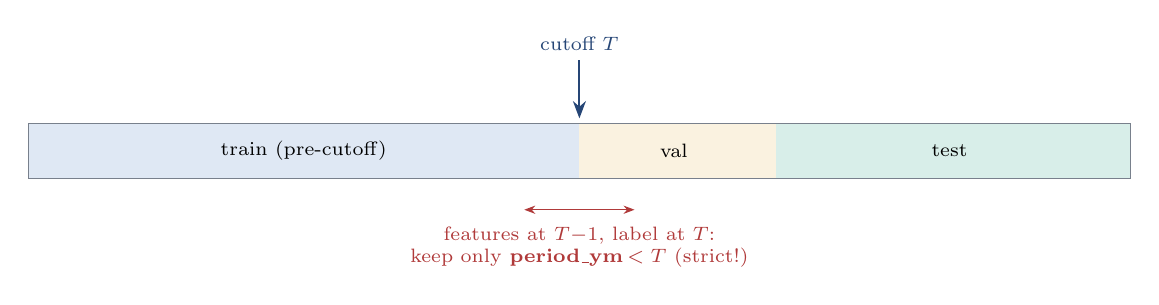
\begin{tikzpicture}[x=1mm,y=1mm]
  \fill[nodeblue] (0,0) rectangle (70,7);
  \fill[nodeamber] (70,0) rectangle (95,7);
  \fill[nodeteal] (95,0) rectangle (140,7);
  \draw[derfr] (0,0) rectangle (140,7);
  \node[font=\scriptsize] at (35,3.5) {train (pre-cutoff)};
  \node[font=\scriptsize] at (82,3.5) {val};
  \node[font=\scriptsize] at (117,3.5) {test};
  \draw[flow, draw=accent] (70,15) -- (70,7.6);
  \node[font=\scriptsize, text=accent, anchor=south] at (70,15) {cutoff $T$};
  \draw[{Stealth[length=1.4mm]}-{Stealth[length=1.4mm]}, draw=plotred] (63,-4) -- (77,-4);
  \node[font=\scriptsize, text=plotred, anchor=north, align=center] at (70,-5)
       {features at $T{-}1$, label at $T$:\\ keep only \textbf{period\_ym}$\,<T$ (strict!)};
\end{tikzpicture}
\caption{The strictly temporal split. Time runs left to right; the model only ever trains on
months before the cutoff and is tested on later months. Because each label looks one month
ahead, an example is admissible only when \texttt{period\_ym}$\,<T$ --- the strict inequality
that prevents the post-cutoff transition from leaking into training.}
\end{figure}

\begin{intuition}[Our cutoff is a genuine design decision --- and a question for the advisor]
Our Fannie Mae data runs roughly 2000--2025, which means our test window can straddle the
COVID shock of 2020--2021, when prepayment and forbearance behaviour was historically
abnormal. A reasonable first choice is to train on pre-2022 data, but the COVID distortion
makes the cutoff a real judgement call rather than a mechanical one: train through the shock
and the model may overfit a once-in-a-generation regime; stop before it and the model never
sees a stress episode. The natural answer is a \emph{rolling backtest} --- repeatedly
retrain up to year $Y$, test on $Y{+}1$, absorb $Y{+}1$, advance --- using the leakage-safe
\texttt{period\_ym}~$<$~cutoff mask. This is exactly the kind of point to settle with Justin
rather than to decide silently.
\end{intuition}

% ======================================================================
\section{Loan-level results: does depth actually help?}
\label{sec:loanresults}

Before the pool, we check the model one loan-month at a time. Two diagnostics matter: overall
fit (cross-entropy loss) and discrimination on specific transitions (AUC).

\subsection{Goodness of fit: the cross-entropy ladder}

The paper reports the out-of-sample loss \eqref{eq:loss} as the network deepens. Lower is
better; this is the same loss we benchmark against the empirical transition matrix.

\begin{table}[H]
\centering
\caption{Out-of-sample loss (negative average log-likelihood) by network depth, from the
original paper. The ensemble is eight five-layer networks.}
\vspace{2pt}
\begin{tabular}{lccc}
\toprule
\textbf{Model} & \textbf{In-sample} & \textbf{Out-of-sample} & \textbf{Out-of-sample} \\
               &                    & (no dropout)           & (with dropout) \\
\midrule
0 hidden layers (logistic) & 0.1840 & 0.1805 & 0.1805 \\
1 hidden layer             & 0.1680 & 0.1700 & 0.1685 \\
3 hidden layers            & 0.1644 & 0.1679 & 0.1671 \\
5 hidden layers            & 0.1639 & 0.1684 & 0.1670 \\
7 hidden layers            & 0.1638 & 0.1688 & 0.1673 \\
\textbf{Ensemble (8$\times$5-layer)} & 0.1640 & \textbf{0.1659} & \textbf{0.1654} \\
\bottomrule
\end{tabular}
\end{table}

\begin{intuition}[How to read this table]
Two lessons. First, depth helps but with diminishing returns: the big jump is from the
linear model (0.1805) to any network at all, and the out-of-sample loss is lowest around
\emph{five} layers with dropout --- deeper is not automatically better, because capacity
also invites overfitting (note the characteristic U-shape). Second, the ensemble beats every
single network: averaging eight five-layer nets gives the best out-of-sample loss of all.
That is why the project's target architecture is ``five layers, ensembled by eight.''
\end{intuition}

\subsection{Discrimination by transition: AUC}

Cross-entropy is one global number; AUC zooms in on individual transitions.

\begin{jargon}[ROC and AUC]
Treat a single transition (say \state{current}~$\to$~\state{prepaid}) as a yes/no
classification: will this loan prepay next month or not? As you sweep the decision
threshold, the model trades off true positives against false positives --- that trade-off
curve is the ROC. The \emph{area under} it (AUC) is a single score in $[0.5, 1]$: 0.5 is a
coin flip, 1 is perfect. Equivalently, AUC is the probability the model scores a true
prepayer above a true non-prepayer.
\end{jargon}

\begin{figure}[H]
\centering
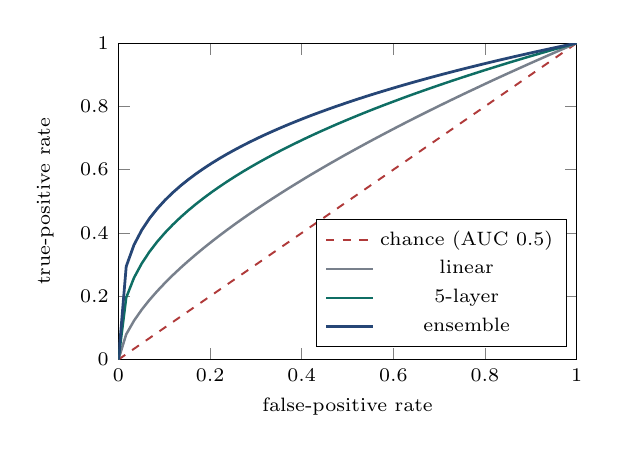
\begin{tikzpicture}
\begin{axis}[width=7.4cm,height=5.6cm, xlabel={false-positive rate}, ylabel={true-positive rate},
  xmin=0,xmax=1,ymin=0,ymax=1, tick label style={font=\scriptsize},
  every axis x label/.style={at={(axis description cs:0.5,-0.09)},anchor=north,font=\scriptsize},
  every axis y label/.style={at={(axis description cs:-0.12,0.5)},rotate=90,anchor=south,font=\scriptsize},
  legend style={font=\scriptsize, at={(0.98,0.04)},anchor=south east}, domain=0:1, samples=60]
  \addplot[plotred, dashed, line width=0.7pt]{x}; \addlegendentry{chance (AUC 0.5)}
  \addplot[derfr, line width=0.9pt]{x^(0.62)}; \addlegendentry{linear}
  \addplot[plotteal, line width=0.9pt]{x^(0.40)}; \addlegendentry{5-layer}
  \addplot[plotblue, line width=1pt]{x^(0.30)}; \addlegendentry{ensemble}
\end{axis}
\end{tikzpicture}
\caption{Illustrative ROC curves for \state{current}~$\to$~\state{prepaid} (schematic, after
the paper's Figure~17). A curve that bows further toward the top-left corner has higher AUC.
The ensemble dominates the single network, which dominates the linear model, which sits only
a little above the chance diagonal.}
\end{figure}

\begin{table}[H]
\centering
\caption{Out-of-sample AUC for transitions \emph{to prepaid}, by depth (original paper).
``dd'' = days delinquent, ``F'' = foreclosure, ``P'' = paid off/prepaid.}
\vspace{2pt}
\begin{tabular}{lccccc}
\toprule
\textbf{Model} & C$\to$P & 30dd$\to$P & 60dd$\to$P & 90+dd$\to$P & F$\to$P \\
\midrule
0 hidden layers & 0.65 & 0.77 & 0.68 & 0.59 & 0.57 \\
1 hidden layer  & 0.72 & 0.79 & 0.71 & 0.76 & 0.68 \\
3 hidden layers & 0.74 & 0.81 & 0.73 & 0.79 & 0.72 \\
5 hidden layers & 0.74 & 0.81 & 0.73 & 0.79 & 0.73 \\
\textbf{Ensemble} & \textbf{0.76} & \textbf{0.83} & \textbf{0.74} & \textbf{0.79} & \textbf{0.74} \\
\bottomrule
\end{tabular}
\end{table}

\begin{intuition}[Where the nonlinearity hides]
Look at \state{90+dpd}~$\to$~\state{prepaid}: the linear model scores a near-useless 0.59,
while a single hidden layer jumps to 0.76 --- a 30\% improvement. The deeper into delinquency,
the more nonlinear the prepayment behaviour, and the more the network adds over logistic
regression. This is the loan-level fingerprint of the same nonlinearity that will make the
pool-level results so different between the two models.
\end{intuition}

\subsection{What the paper actually found (the headline results)}

Beyond the loss and AUC tables, three substantive findings emerge from the paper's analysis,
and they are the ones our replication is really testing.

\begin{keyidea}[Three facts the paper established]
\begin{enumerate}[leftmargin=1.4em, itemsep=2pt]
  \item \textbf{Balance and dynamic variables dominate prepayment.} Loan-balance variables
        outrank the classic static characteristics; the refinancing incentive and house-price
        changes matter more than FICO or LTV (the importance table in
        Section~\ref{sec:features}).
  \item \textbf{Borrower behaviour is highly path-dependent.} For delinquency transitions, the
        recent count of missed payments dominates --- standard loan and borrower characteristics
        are \emph{less} predictive of delinquency than the prior literature assumed.
  \item \textbf{Unemployment's role is real.} The paper firmly establishes the economic
        significance of state unemployment for transitions, a variable earlier (smaller-sample)
        studies had dismissed --- evidence that common macro factors drive correlated,
        pool-level risk.
\end{enumerate}
These are exactly the claims a flexible model can express and a linear one cannot, and they set
up the pool-level payoff in Section~\ref{sec:pool}.
\end{keyidea}

\begin{intuition}[Where our own numbers will go]
The tables in this section report the \emph{paper's} published results --- the benchmark our
replication is measured against, not our own fitted numbers (those are still being computed on
the Fannie Mae panel). When the rolling backtest completes, our loss-by-depth, AUC-by-origin,
and reliability results drop straight into these same exhibits as additional columns, and the
gradient-boosted-tree challenger of Section~\ref{sec:gbt} joins them as one more. The structure
is built to receive the numbers; only the cells are pending.
\end{intuition}

\subsection{What we realistically expect to replicate}

\begin{intuition}[Honest expectations]
Our absolute loss numbers will not match the paper's to the third decimal, and they
should not: different dataset (Fannie Mae, not CoreLogic), different and initially smaller
feature set (macro covariates are out of scope for the first pass), a different and more
recent time span. What we expect to reproduce is the \emph{shape} of the findings: networks
beat logistic regression and the empirical-matrix benchmark; five layers ensembled is near
the sweet spot; and the gains concentrate in prepayment and in transitions out of severe
delinquency. The qualitative story is the replication; the exact digits are not.
\end{intuition}

% ======================================================================
\section{Pool-level prediction: the result that matters most}
\label{sec:pool}

This is the section to read twice. Everything so far has been at the level of a single
loan-month. Now we aggregate to a \emph{pool} --- a thousand loans bundled together --- which
is the object that mortgage-backed securities are written on. The punchline of the whole
dissertation lives here: \emph{the nonlinearities that help a little per loan compound into a
large, decisive advantage at the pool level.}

\subsection{Why pools, and why investors care}

\begin{jargon}[MBS, and pool-level risk]
A mortgage-backed security (MBS) bundles many mortgages and sells investors the right to the
combined cash flows. The investor does not care about any one borrower; they care about how
many loans in the pool \emph{prepay} (returning principal early, to be reinvested at lower
rates) or \emph{default}. Pool-level prepayment and delinquency rates are exactly what drive
MBS value. So a model that forecasts the \emph{pool} accurately is directly a model that
prices MBS accurately.
\end{jargon}

\subsection{The crux: a pool prediction is a sum, not a new model}

\begin{keyidea}[There is no pool-level model]
The expected behaviour of a pool is just the sum of the expected behaviours of its loans.
For a pool of $N$ loans and a 12-month horizon,
\begin{equation}
  \underbrace{\text{predicted \# prepayments}}_{\text{pool-level}}
  \;=\; \sum_{i=1}^{N} \Prob\!\left(\text{loan } i \text{ prepays within 12 months}\right),
  \label{eq:poolsum}
\end{equation}
where each loan's probability comes from the \emph{same} loan-level transition network, rolled
forward 12 months. We never fit a separate pool model. Pool predictions are a pure
cross-sectional sum of loan-level outputs.
\end{keyidea}

\begin{intuition}[Why this is the whole game]
Because the pool prediction is built by addition, two things follow immediately. Accuracy is
inherited: a better loan-level model gives a better pool-level model for free. And
\emph{bias} is inherited too: if the loan-level model systematically over-predicts
prepayment, those errors do not cancel across loans --- they pile up in the sum. That second
fact is precisely why the linear model fails at the pool level, as we will see.
\end{intuition}

\subsection{The roll-forward, explained slowly}

Equation \eqref{eq:poolsum} needs ``the probability loan $i$ prepays within 12 months.'' Our
network only directly predicts \emph{one month ahead}. So we must roll it forward. This is the
step worth pinning down precisely.

\textbf{Step 1 --- one month is a matrix.} For loan $i$ in month $m$, the network turns its
features into a full next-state distribution for \emph{every} possible current state. Collect
these into a $7\times 7$ \emph{conditional transition matrix} $P^{(i)}_m$, whose $(u,v)$ entry
is
\[
  \bigl(P^{(i)}_m\bigr)_{u,v} \;=\; h_\theta\!\left(v \,\middle|\, u,\; x^{(i)}_m\right)
  \;=\; \Prob(\text{state } v \text{ next month} \mid \text{state } u \text{ now}).
\]
Each row is a probability distribution (it sums to 1). \state{prepaid} and \state{REO} are
\emph{absorbing}: their rows put all mass on themselves.

\textbf{Step 2 --- represent ``where the loan is'' as a vector.} Let $\pi^{(i)}_0$ be a
length-7 one-hot row vector with a 1 in the loan's current state. Multiplying a state
distribution by the transition matrix advances it one month:
\[
  \pi^{(i)}_{1} \;=\; \pi^{(i)}_0\, P^{(i)}_0 .
\]

\textbf{Step 3 --- chain twelve of them.} Twelve months ahead is twelve matrix multiplications:
\begin{equation}
  \pi^{(i)}_{12}
  \;=\; \pi^{(i)}_0 \; P^{(i)}_0\, P^{(i)}_1\, \cdots\, P^{(i)}_{11}.
  \label{eq:rollforward}
\end{equation}
The probability loan $i$ has prepaid by month 12 is simply the \state{prepaid} entry of
$\pi^{(i)}_{12}$ --- and because \state{prepaid} is absorbing, that entry is exactly the
cumulative chance of \emph{ever} prepaying within the year.

\begin{keyidea}[Answering the roll-forward question directly]
You do \textbf{not} ask the network for a 12-month probability in one shot. You ask it for
\emph{this} month, get a $7\times 7$ matrix, step the state vector forward, and repeat twelve
times. Twelve one-month predictions chained together \emph{are} the twelve-month prediction.
Equation \eqref{eq:rollforward} is the entire roll-forward.
\end{keyidea}

\begin{figure}[H]
\centering
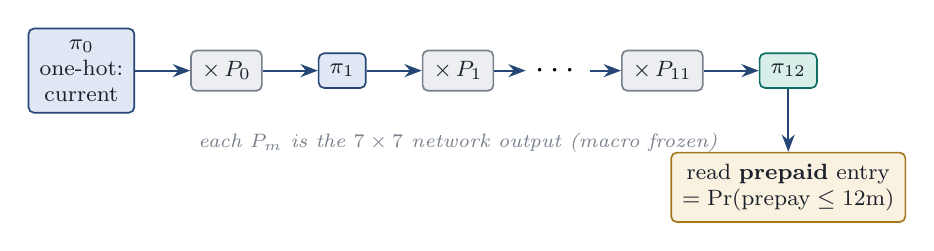
\begin{tikzpicture}[node distance=5mm and 7mm]
  \node[box] (p0) {$\pi_0$\\one-hot:\\current};
  \node[gbox, right=of p0] (m0) {$\times\,P_0$};
  \node[box, right=of m0] (p1) {$\pi_1$};
  \node[gbox, right=of p1] (m1) {$\times\,P_1$};
  \node[font=\large, right=4mm of m1] (dots) {$\cdots$};
  \node[gbox, right=4mm of dots] (m11) {$\times\,P_{11}$};
  \node[tbox, right=of m11] (p12) {$\pi_{12}$};
  \draw[flow] (p0)--(m0); \draw[flow] (m0)--(p1); \draw[flow] (p1)--(m1);
  \draw[flow] (m1)--(dots); \draw[flow] (dots)--(m11); \draw[flow] (m11)--(p12);
  \node[abox, below=8mm of p12, align=center] (read)
       {read \textbf{prepaid} entry\\$=\Pr(\text{prepay}\le 12\text{m})$};
  \draw[flow] (p12)--(read);
  \node[font=\scriptsize\itshape, text=derfr, below=4mm of m1, align=center]
       {each $P_m$ is the $7\times7$ network output (macro frozen)};
\end{tikzpicture}
\caption{The roll-forward, the step that the loan-level network does \emph{not} do directly.
Start from a one-hot state vector $\pi_0$, multiply by twelve successive one-month transition
matrices $P_0,\dots,P_{11}$ (each produced by the network from the loan's features that month,
with macro variables frozen), and read off the \texttt{prepaid} coordinate of $\pi_{12}$.
Because \texttt{prepaid} is absorbing, that coordinate is the cumulative probability of having
prepaid within the year.}
\end{figure}

This chaining is an instance of the \emph{Chapman--Kolmogorov} identity for Markov chains: the
$t$-step transition matrix is the product of the one-step matrices,
\begin{equation}
  P^{(0\to t)} \;=\; P_0\,P_1\cdots P_{t-1},
  \label{eq:chapman}
\end{equation}
and the loan's $t$-month state distribution is $\pi_t = \pi_0\, P^{(0\to t)}$.

\begin{derivation}[Why multiplying matrices advances time]
Entry $(u,v)$ of the product $P_0 P_1$ is $\sum_{w}(P_0)_{u,w}(P_1)_{w,v}$ --- the
probability of going $u\to w$ in month 0 \emph{and then} $w\to v$ in month 1, summed over
every possible intermediate state $w$. That sum-over-paths is exactly the law of total
probability across the unobserved middle state, and iterating it twelve times sums over all
twelve-month trajectories at once. So a single matrix product silently accounts for every way
a loan could wander through delinquency and back before (or instead of) prepaying.
\end{derivation}

\textbf{What changes between the twelve months?} Two options:

\begin{enumerate}[leftmargin=1.6em, itemsep=2pt]
  \item \textbf{Frozen covariates (the cheap, accurate-for-12-months choice).} Freeze the
        macro variables (rates, prices, unemployment) at their month-0 values. Only the loan's
        own deterministic features evolve --- its scheduled balance, its age, its remaining
        term --- and its state, which is what the $\pi$ vector tracks. Then the matrices in
        \eqref{eq:rollforward} are deterministic and you just multiply them. This is how the
        paper produces the point predictions in the scatter plots.
  \item \textbf{Simulated covariates (for the full distribution).} Treat the macro variables
        as random, simulate many future paths, recompute the matrices along each path, and
        average. This is more expensive but yields a whole \emph{distribution} of pool
        outcomes, not just a mean (next subsection).
\end{enumerate}

\begin{intuition}[Why freezing is legitimate over a year]
Over twelve months, a borrower's state can swing a lot, but the national mortgage rate and
local prices move comparatively slowly. Freezing them introduces only a small error at the
one-year horizon while removing the need to model their joint dynamics --- a very favourable
trade for the point estimate. For the \emph{distribution}, though, the spread is mostly driven
by where rates go, so there we must let the rate move.
\end{intuition}

\subsection{Building the pools}

To stress-test the model across risk levels, the paper builds pools that deliberately differ
in quality. Take 2 million test loans, \textbf{sort} them by a chosen characteristic, and
chop the sorted list into consecutive blocks of 1{,}000 --- giving 2{,}000 pools that range
smoothly from low to high risk. Four sorting keys are used:

\begin{center}
FICO score \quad$\bullet$\quad original interest rate \quad$\bullet$\quad LTV ratio
\quad$\bullet$\quad predicted probability of staying current.
\end{center}

(Our project mirrors the first three.) For each pool, the predicted prepayment count is the
sum \eqref{eq:poolsum} of its 1{,}000 loans' rolled-forward probabilities, and the observed
count is what actually happened in the test data over the next 12 months.

\begin{figure}[H]
\centering
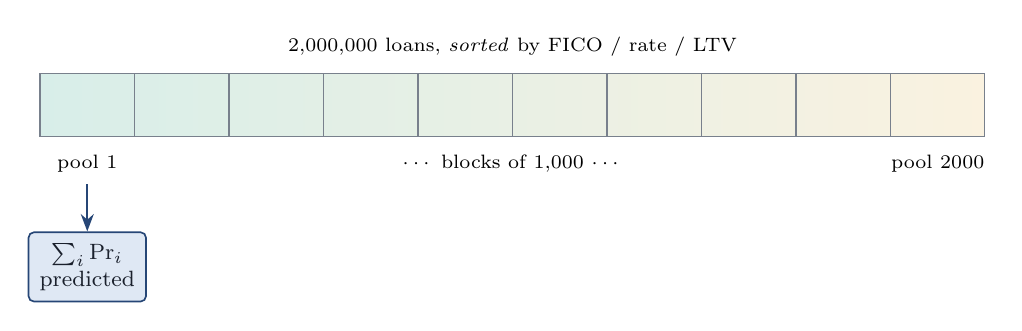
\begin{tikzpicture}[x=1mm,y=1mm]
  \shade[left color=nodeteal, right color=nodeamber] (0,0) rectangle (120,8);
  \draw[derfr] (0,0) rectangle (120,8);
  \foreach \x in {12,24,36,...,108} \draw[derfr] (\x,0)--(\x,8);
  \node[font=\scriptsize,anchor=south] at (60,9) {2{,}000{,}000 loans, \emph{sorted} by FICO / rate / LTV};
  \node[font=\scriptsize,anchor=north] at (6,-1) {pool 1};
  \node[font=\scriptsize,anchor=north] at (114,-1) {pool 2000};
  \node[font=\scriptsize,anchor=north] at (60,-1) {$\cdots$ blocks of 1{,}000 $\cdots$};
  \draw[flow] (6,-6) -- (6,-12);
  \node[box, anchor=north, align=center] at (6,-12) {$\sum_i \Pr_i$\\predicted};
\end{tikzpicture}
\caption{Building pools of graded risk. Sort all loans by a characteristic, then chop the
sorted list into consecutive blocks of 1{,}000. Pools then range smoothly from low to high
risk, and each pool's prediction is just the sum of its loans' rolled-forward probabilities.}
\end{figure}

\subsection{The headline picture: observed vs.\ predicted}

Plot each pool as a point: observed prepayments on the $x$-axis, predicted on the $y$-axis.
Perfect prediction lies on the 45-degree line $y=x$.

\begin{intuition}[What the scatter shows --- and it is striking]
The five-layer network's points hug the $y=x$ line across the whole range of pool risk. The
linear zero-layer model's points sit \emph{systematically above} the line --- it persistently
over-predicts prepayment, and the bias does not wash out. The difference is not subtle, and it
is the visual heart of the dissertation.
\end{intuition}

\begin{figure}[H]
\centering
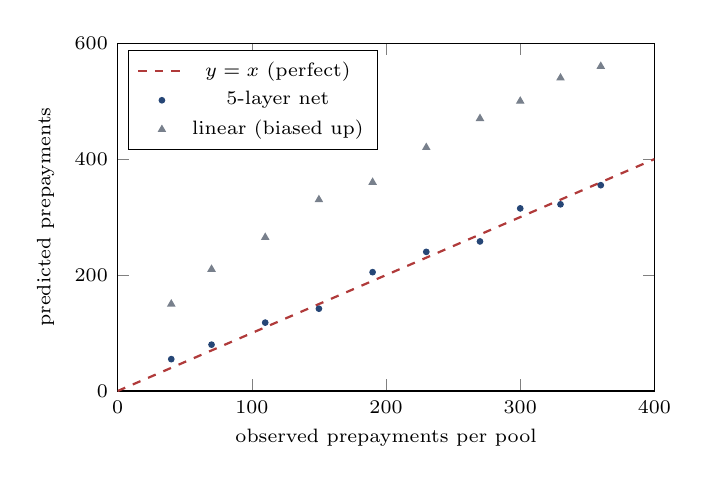
\begin{tikzpicture}
\begin{axis}[width=8.4cm,height=6cm, xlabel={observed prepayments per pool},
  ylabel={predicted prepayments}, xmin=0,xmax=400,ymin=0,ymax=600,
  every axis x label/.style={at={(axis description cs:0.5,-0.08)},anchor=north,font=\scriptsize},
  every axis y label/.style={at={(axis description cs:-0.1,0.5)},rotate=90,anchor=south,font=\scriptsize},
  tick label style={font=\scriptsize}, legend style={font=\scriptsize, at={(0.02,0.98)},anchor=north west}]
  \addplot[domain=0:400, plotred, dashed, line width=0.8pt]{x}; \addlegendentry{$y=x$ (perfect)}
  \addplot[only marks, mark=*, mark size=1pt, plotblue] coordinates {
    (40,55)(70,80)(110,118)(150,142)(190,205)(230,240)(270,258)(300,315)(330,322)(360,355)};
  \addlegendentry{5-layer net}
  \addplot[only marks, mark=triangle*, mark size=1.4pt, derfr] coordinates {
    (40,150)(70,210)(110,265)(150,330)(190,360)(230,420)(270,470)(300,500)(330,540)(360,560)};
  \addlegendentry{linear (biased up)}
\end{axis}
\end{tikzpicture}
\caption{Out-of-sample pool predictions (schematic, after the paper's Figures~19--22). Each
point is one pool: observed prepayments on the $x$-axis, model-predicted on the $y$-axis.
The network's points track the perfect-prediction line; the linear model's points lie
consistently above it --- a bias that, crucially, does not cancel out across pools.}
\end{figure}

\begin{table}[H]
\centering
\caption{Out-of-sample pool-level distribution, averaged over 50 test portfolios of 10{,}000
loans each, one-year horizon (original paper, Table 22). ``Standardised gap'' is the
prediction error in units of the forecast's own standard deviation.}
\vspace{2pt}
\begin{tabular}{lcc}
\toprule
 & \textbf{0-layer (linear)} & \textbf{5-layer network} \\
\midrule
Avg.\ actual prepayments     & 1723.8 & 1723.8 \\
Avg.\ predicted prepayments  & 2853.8 & \textbf{1456.9} \\
Avg.\ absolute gap           & 1186.0 & \textbf{278.5} \\
Avg.\ standardised gap       & 2.4    & \textbf{1.9} \\
\bottomrule
\end{tabular}
\end{table}

\begin{intuition}[Reading Table 22 --- the single most quotable result]
The truth is about \textbf{1724} prepayments per pool. The linear model predicts
\textbf{2854} --- a 1186-prepayment error, two-thirds too high. The five-layer network predicts
\textbf{1457} --- an error of 279, more than \emph{four times} smaller. The network is not
perfect (it slightly under-predicts here), but it is dramatically closer, and its forecast
distribution is tighter too. For an MBS investor pricing cash flows, that is the difference
between a usable model and a misleading one.
\end{intuition}

\subsection{The full distribution, via Monte Carlo on rates}

For a richer view, the paper simulates the \emph{distribution} of a pool's prepayments rather
than a single number. The recipe:

\begin{enumerate}[leftmargin=1.6em, itemsep=2pt]
  \item Fit a small time-series model to the national mortgage rate --- an AR(4) on the
        Freddie Mac series (the same family as our PMMS feature).
  \item Simulate many future rate paths from that AR(4); freeze the other macro variables.
  \item Along each path, recompute every loan's roll-forward \eqref{eq:rollforward} and sum
        to a pool prepayment count.
  \item The spread of those counts across paths is the forecast \emph{distribution}.
\end{enumerate}

\begin{jargon}[AR(4)]
An autoregressive model of order 4: next period's rate is a linear function of the previous
four periods' rates plus noise. It is a compact way to generate plausible random future
interest-rate paths so that correlated prepayment --- everyone refinancing at once when rates
drop --- is captured. The paper's fitted coefficients (intercept and four lags) are
$[\,0.6687,\; 1.3514,\; -0.5131,\; 0.2410,\; -0.0838\,]$, with the lag length chosen from the
partial-autocorrelation plot --- a deliberately simple model whose only job is to generate
realistic rate scenarios.
\end{jargon}

\begin{intuition}[The tell-tale sign of a good model]
For the five-layer network, the \emph{actually observed} prepayment count lands near the
\emph{centre} of the simulated distribution --- the model's uncertainty is well-calibrated.
For the linear model, the observed count falls out in the \emph{tail} --- reality is an event
the linear model thought was unlikely. A model that is routinely surprised by reality is the
wrong model to price a security with.
\end{intuition}

When the macro covariates are \emph{frozen}, the loans become conditionally independent and
the pool prepayment count $S = \sum_{i=1}^N B_i$ is a sum of independent Bernoulli indicators
$B_i$ (loan $i$ prepays or not), with $\Pr(B_i=1)=p_i$. Its mean and variance are then
exactly
\begin{equation}
  \E[S] \;=\; \sum_{i=1}^N p_i,
  \qquad
  \operatorname{Var}(S) \;=\; \sum_{i=1}^N p_i(1-p_i),
  \label{eq:poolmoments}
\end{equation}
and for a pool of hundreds or thousands of loans the central limit theorem makes $S$
approximately Normal (equivalently, a Poisson approximation applies when the $p_i$ are small).

\begin{derivation}[Why a few hundred loans already give a tight forecast]
The mean prediction \eqref{eq:poolmoments} is the same sum \eqref{eq:poolsum} we have used
throughout. The new content is the \emph{variance}: it grows like $N$ while the mean also
grows like $N$, so the relative spread $\sqrt{\operatorname{Var}(S)}/\E[S]$ shrinks like
$1/\sqrt{N}$. That is why the paper can say closed-form Normal/Poisson approximations are
accurate ``even for pools with only a few hundred loans'': pooling averages away
idiosyncratic loan-level uncertainty. What it does \emph{not} average away is the shared
macro risk --- which is precisely why the full distribution (previous subsection) must
simulate the rate path rather than freeze it.
\end{derivation}

\begin{figure}[H]
\centering
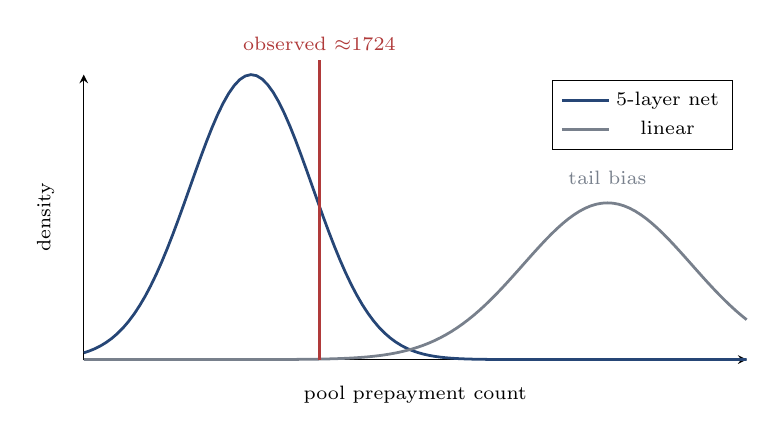
\begin{tikzpicture}
\begin{axis}[width=10cm,height=5.2cm, xlabel={pool prepayment count},
  ylabel={density}, xtick=\empty, ytick=\empty, axis lines=left, domain=800:3400, samples=120,
  every axis x label/.style={at={(axis description cs:0.5,-0.06)},anchor=north,font=\scriptsize},
  every axis y label/.style={at={(axis description cs:-0.03,0.5)},rotate=90,anchor=south,font=\scriptsize},
  clip=false, legend style={font=\scriptsize, at={(0.98,0.98)},anchor=north east}]
  \addplot[plotblue, line width=1pt]{exp(-(x-1457)^2/(2*240^2))};
  \addlegendentry{5-layer net}
  \addplot[derfr, line width=1pt]{0.55*exp(-(x-2854)^2/(2*330^2))};
  \addlegendentry{linear}
  \draw[plotred, line width=0.9pt] (axis cs:1724,0) -- (axis cs:1724,1.05);
  \node[font=\scriptsize, text=plotred, anchor=south] at (axis cs:1724,1.05) {observed $\approx$1724};
  \node[font=\scriptsize, text=derfr, anchor=south] at (axis cs:2854,0.58) {tail bias};
\end{axis}
\end{tikzpicture}
\caption{Forecast distributions of pool prepayments (schematic, after the paper's
Figures~23--24 and Table~22). The network's distribution is narrow and brackets the observed
outcome; the linear model's distribution is shifted far to the right, leaving the truth in its
left tail. Numbers echo Table~22: linear mean $\approx$2854, network mean $\approx$1457,
observed $\approx$1724.}
\end{figure}

\subsection{Why the linear model is biased and the network is not}

\begin{derivation}[The mechanism, spelled out]
The pool prediction \eqref{eq:poolsum} sums one probability per loan. If each loan's
probability were \emph{unbiased}, the per-loan errors would be roughly independent and would
average out --- the law of large numbers would make the pool sum very accurate. But the linear
model is \emph{mis-specified} for prepayment: it cannot represent the S-shaped incentive curve
or the FICO plateau, so it makes errors with a \emph{consistent sign}. Worse, every loan in
the pool shares the same macro covariates (one national rate, one local price path), so when
the linear model mis-reads that shared environment, it mis-reads it \emph{the same way for
every loan at once}. The errors are correlated, they all point the same direction, and the sum
amplifies them instead of cancelling them. The network, by fitting the true nonlinear shape,
keeps each loan's probability close to unbiased --- so the sum stays accurate. This is the
deep reason a small per-loan edge becomes a large per-pool edge.
\end{derivation}

\begin{keyidea}[The dissertation's thesis, restated at the pool level]
Capturing the nonlinearities in borrower behaviour does not just sharpen individual-loan
forecasts; it removes a \emph{systematic, correlated bias} from pool-level forecasts. Because
MBS are priced off pool-level cash flows, that bias removal translates directly into more
accurate MBS valuation --- which is the practical pay-off the whole exercise is aiming at.
\end{keyidea}

% ======================================================================
\section{A non-neural challenger: gradient-boosted trees}
\label{sec:gbt}

Everything so far has pitted one flexible model (the neural network) against one rigid one
(logistic regression). The network won. But that raises a sharper question the dissertation
can answer, and which the original paper never asked: \emph{when the flexible model wins, is
it winning because it is flexible, or because it is \textbf{smooth}?} To separate those two
explanations we add a second flexible learner with the \emph{opposite} inductive bias ---
gradient-boosted trees --- and race it against the net. This section explains what that
learner is, why we chose it over the alternatives we considered, where it slots into the
machine we have already built, and what each possible outcome of the race would teach us.

\subsection{The question GBT is built to answer}

\begin{keyidea}[Flexibility vs.\ smoothness]
The neural network is \emph{flexible} (it can fit complicated surfaces) \emph{and} \emph{smooth}
(it is biased toward gently-curving functions). Logistic regression is neither. So ``the net
beats logit'' confounds the two virtues. A gradient-boosted tree ensemble is just as flexible
as the net but is \emph{not} smooth --- it builds its predictions out of sharp, axis-aligned
steps. Racing net against GBT therefore holds flexibility roughly fixed and varies smoothness,
isolating \emph{which kind of flexibility} the mortgage-transition surface actually rewards.
\end{keyidea}

\subsection{What a decision tree is}

The atom of the challenger is the \textbf{decision tree}. A tree asks a sequence of yes/no
questions about the features --- ``is FICO below 660?'', then ``is the rate incentive above
1\%?'' --- and each path down the tree ends in a \emph{leaf} that emits a constant prediction.

\begin{figure}[H]
\centering
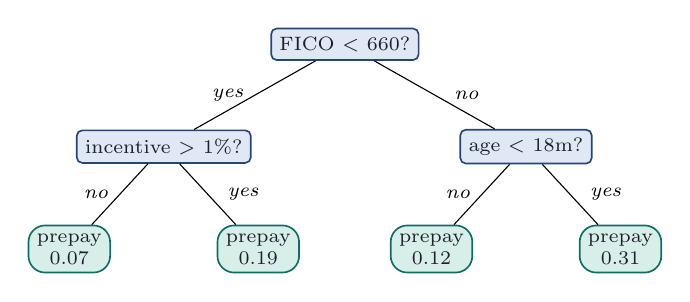
\begin{tikzpicture}[level distance=13mm, level 1/.style={sibling distance=46mm},
  level 2/.style={sibling distance=24mm}]
\node[split] {FICO $<$ 660?}
  child {node[split] {incentive $>$ 1\%?}
    child {node[leaf] {prepay\\0.07} edge from parent node[left,font=\scriptsize\itshape,inner sep=1pt]{no\ \ }}
    child {node[leaf] {prepay\\0.19} edge from parent node[right,font=\scriptsize\itshape,inner sep=1pt]{\ \ yes}}
    edge from parent node[left,font=\scriptsize\itshape,inner sep=1pt]{yes\ \ }}
  child {node[split] {age $<$ 18m?}
    child {node[leaf] {prepay\\0.12} edge from parent node[left,font=\scriptsize\itshape,inner sep=1pt]{no\ \ }}
    child {node[leaf] {prepay\\0.31} edge from parent node[right,font=\scriptsize\itshape,inner sep=1pt]{\ \ yes}}
    edge from parent node[right,font=\scriptsize\itshape,inner sep=1pt]{\ \ no}};
\end{tikzpicture}
\caption{A single (tiny) decision tree. Internal nodes split on one feature at a time; leaves
give a constant predicted probability. A path that splits on FICO \emph{and then} on incentive
has automatically captured an \emph{interaction} between them --- the effect of incentive differs
depending on the FICO branch.}
\end{figure}

Mathematically a tree partitions the feature space into rectangular regions $R_1,\dots,R_J$ and
predicts a constant $c_j$ in each:
\begin{equation}
  f(x) \;=\; \sum_{j=1}^{J} c_j\, \mathbf{1}\{x \in R_j\}.
  \label{eq:tree}
\end{equation}

\begin{intuition}[What trees are naturally good and bad at]
Three things come for free: trees are \emph{scale-invariant} (only the order of a feature's
values matters, so no standardisation is needed --- contrast equation~\eqref{eq:standardize});
they handle missing values and categoricals like origin \texttt{state} natively; and they
capture interactions automatically by stacking splits. The cost is the shape of
\eqref{eq:tree}: the prediction is \emph{piecewise constant}, a landscape of flat plateaus with
vertical cliffs between them. A single tree is also high-variance --- redraw the data and the
splits jump around. Boosting fixes the variance; the piecewise-constant shape is intrinsic, and
it is the whole point of the comparison.
\end{intuition}

\subsection{From one tree to a boosted ensemble}

A single shallow tree is a weak model. \textbf{Gradient boosting} turns many weak trees into a
strong one by building them \emph{sequentially}, each new tree correcting the errors the running
ensemble has made so far. The model is an additive sum,
\begin{equation}
  F_M(x) \;=\; \sum_{m=1}^{M} \nu\, h_m(x),
  \qquad
  F_m = F_{m-1} + \nu\, h_m,
  \label{eq:boost}
\end{equation}
where each $h_m$ is a tree and $\nu$ is a small \emph{learning rate} that shrinks each tree's
contribution so the ensemble improves in cautious steps.

\begin{figure}[H]
\centering
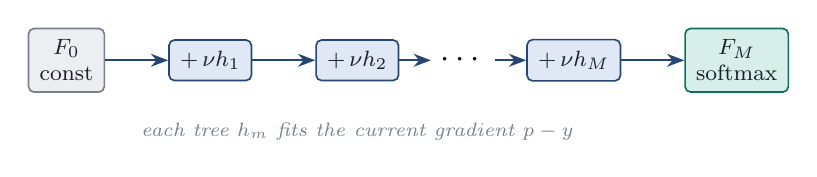
\begin{tikzpicture}[node distance=5mm and 8mm]
  \node[gbox] (f0) {$F_0$\\const};
  \node[box, right=of f0] (t1) {$+\,\nu h_1$};
  \node[box, right=of t1] (t2) {$+\,\nu h_2$};
  \node[font=\large, right=4mm of t2] (d) {$\cdots$};
  \node[box, right=4mm of d] (tm) {$+\,\nu h_M$};
  \node[tbox, right=of tm] (fm) {$F_M$\\softmax};
  \draw[flow] (f0)--(t1); \draw[flow] (t1)--(t2); \draw[flow] (t2)--(d);
  \draw[flow] (d)--(tm); \draw[flow] (tm)--(fm);
  \node[font=\scriptsize\itshape, text=derfr, below=4mm of t2, align=center]
    {each tree $h_m$ fits the current gradient $p-y$};
\end{tikzpicture}
\caption{Gradient boosting. Start from a constant, then add one shrunken tree at a time, each
fitted to the direction that most reduces the loss. The final ensemble passes through a softmax
so its seven outputs are a valid probability distribution --- exactly what the roll-forward and
cashflow engines require.}
\end{figure}

The word ``gradient'' is literal: each tree $h_m$ is fitted to the \emph{negative gradient} of
the loss with respect to the current predictions --- the direction in which nudging the
predictions would most reduce the loss. And here a familiar face returns.

\begin{derivation}[The same $p-y$ gradient as the net]
With the multiclass softmax cross-entropy loss --- the \emph{same} loss the network minimises ---
the gradient with respect to each class's score is once again
\[
  g_k \;=\; p_k - y_k,
  \qquad\text{with curvature (Hessian) } \; H_{kk} = p_k(1-p_k),
\]
exactly equation~\eqref{eq:pmy} from the network's output layer. So each boosting round fits
seven trees (one per class) to the residual ``predicted minus actual,'' and uses the curvature
to set each leaf's value by a Newton step, $c_j \approx -\sum g \,/\,(\sum H + \lambda)$. The
profound point: \textbf{the net and GBT minimise the identical objective with the identical
gradient signal.} They differ in one thing only --- the \emph{class of functions} each searches
to represent that signal: smooth compositions of ReLU layers for the net, sums of axis-aligned
step functions for GBT.
\end{derivation}

\begin{jargon}[LightGBM, and why this particular implementation]
\emph{LightGBM} is a fast, memory-light gradient-boosting library. Two features make it the
practical choice here. It \emph{bins} each continuous feature into a histogram (e.g.\ 255 bins),
so a row stores one byte per feature and the whole thinned training set --- tens of millions of
rows --- fits in a couple of gigabytes of RAM. And it grows trees \emph{leaf-wise} (splitting
wherever the loss drops most) rather than level-by-level, reaching lower loss in fewer splits.
For a 7-class problem it builds seven trees per round, the source of a roughly $7\times$
wall-clock factor.
\end{jargon}

\begin{intuition}[Is it actually cheap? The numbers say yes]
The ``almost free'' claim is concrete. LightGBM's binned dataset stores one byte per
feature-value, so our thinned $\sim$74\,M\,$\times\,$30 training slice occupies roughly
$\mathbf{2.2}$\,\textbf{GB} of RAM, versus $\sim$17.8\,GB for a raw float64 copy --- it fits on
any laptop. On its published benchmark LightGBM trains a 10.5\,M\,$\times$\,28 dataset in about
$\mathbf{130}$\,\textbf{seconds} on 16 cores; scaling for our row count and the $7\times$
multiclass multiplier puts a full window at an estimated $\sim$1.5--2.5 hours (an
extrapolation, flagged as such), so all eleven backtest windows are a single overnight CPU job.
And the GPU barely helps: at $\sim$30 features LightGBM's leaf-wise growth is sequential and
measured GPU speedups are around $1\times$ (often slower), so the whole leg runs for \$0 on the
Apple-Silicon Mac, or a few dollars on a cheap CPU pod --- leaving the scarce GPU credit for net
re-runs. Compared with training and ensembling the neural network, the challenger is a rounding
error on the compute budget.
\end{intuition}

\subsection{Two flexibilities, opposite biases}

We can now see the crux of the whole comparison in a single picture. Take the smooth prepayment
S-curve from Section~\ref{sec:features}. The net, biased toward smoothness, traces it with a
gentle curve. GBT, built from steps, can only \emph{approximate} it with a staircase --- and to
make the staircase fine it needs many splits, paying in variance and, crucially, in the accuracy
of the probability \emph{levels} the pool valuation consumes.

\begin{figure}[H]
\centering
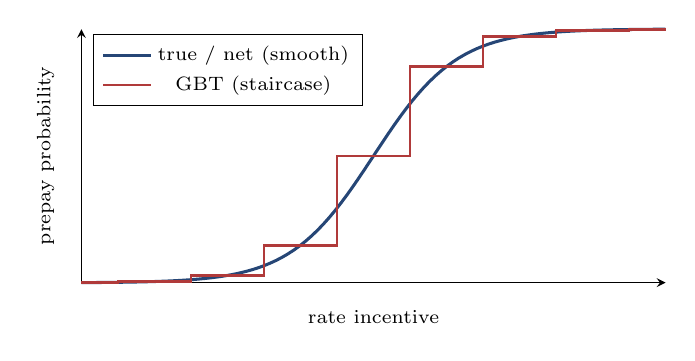
\begin{tikzpicture}
\begin{axis}[width=9cm,height=4.8cm, xlabel={rate incentive}, ylabel={prepay probability},
  xtick=\empty, ytick=\empty, axis lines=left, domain=-4:6, clip=false,
  every axis x label/.style={at={(axis description cs:0.5,-0.07)},anchor=north,font=\scriptsize},
  every axis y label/.style={at={(axis description cs:-0.03,0.5)},rotate=90,anchor=south,font=\scriptsize},
  legend style={font=\scriptsize, at={(0.02,0.98)},anchor=north west}]
  \addplot[plotblue, line width=1.1pt, samples=100]{0.06+0.5/(1+exp(-1.4*(x-1)))};
  \addlegendentry{true / net (smooth)}
  \addplot[plotred, line width=1pt, const plot mark mid, samples=9]{0.06+0.5/(1+exp(-1.4*(x-1)))};
  \addlegendentry{GBT (staircase)}
\end{axis}
\end{tikzpicture}
\caption{The inductive-bias contrast in one dimension. A smooth target (the prepayment
incentive curve) is traced gracefully by a smooth learner and only \emph{stepped through} by a
tree ensemble. Where the economically important structure is smooth, the staircase is at a
disadvantage; where it is genuinely jumpy (policy thresholds, vintage cliffs), the staircase can
win. Which effect dominates on this panel is an empirical question.}
\end{figure}

The same contrast in two feature dimensions: a tree carves the space into axis-aligned boxes,
while the net draws a smooth, possibly diagonal, boundary.

\begin{figure}[H]
\centering
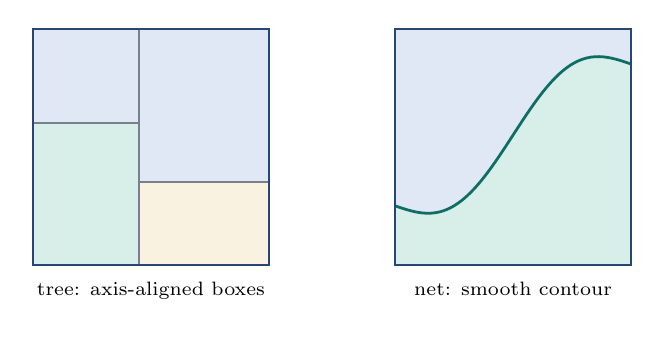
\begin{tikzpicture}[x=30mm,y=30mm]
  \begin{scope}
    \fill[nodeblue] (0,0) rectangle (1,1);
    \fill[nodeteal] (0,0) rectangle (0.45,0.6);
    \fill[nodeamber] (0.45,0) rectangle (1,0.35);
    \draw[edge] (0.45,0)--(0.45,1);
    \draw[edge] (0,0.6)--(0.45,0.6);
    \draw[edge] (0.45,0.35)--(1,0.35);
    \draw[accent,line width=0.7pt] (0,0) rectangle (1,1);
    \node[font=\scriptsize, below=1mm] at (0.5,0) {tree: axis-aligned boxes};
  \end{scope}
  \begin{scope}[xshift=46mm]
    \fill[nodeteal] (0,0) rectangle (1,1);
    \begin{scope}
      \clip (0,0) rectangle (1,1);
      \fill[nodeblue] plot[domain=0:1,samples=60] (\x, {0.25+0.6*\x-0.15*sin(360*\x)}) -- (1,1) -- (0,1) -- cycle;
    \end{scope}
    \draw[accent2,line width=1pt] plot[domain=0:1,samples=60] (\x,{0.25+0.6*\x-0.15*sin(360*\x)});
    \draw[accent,line width=0.7pt] (0,0) rectangle (1,1);
    \node[font=\scriptsize, below=1mm] at (0.5,0) {net: smooth contour};
  \end{scope}
\end{tikzpicture}
\caption{Decision boundaries over two features (say FICO and incentive). The tree can only cut
parallel to the axes, tiling the plane with rectangles; the network can bend a smooth boundary
in any direction. Both are flexible; their flexibility has a different \emph{grain}.}
\end{figure}

\begin{keyidea}[Same capacity, opposite bias --- a controlled experiment]
Because the net and GBT have comparable capacity but opposite inductive bias, a net-vs-GBT gap
is attributable to the \emph{kind} of flexibility, not the \emph{amount}. That is what upgrades
the dissertation's claim from the generic ``flexible beats linear'' to the specific and more
interesting ``the prime-conforming transition surface rewards \emph{smooth} flexibility.''
\end{keyidea}

\subsection{Why GBT, and not the other candidates}

GBT was not the only non-neural learner we could have added. We considered several and
deliberately dispatched them; recording that reasoning is part of the contribution, because the
choice of a single, well-justified challenger is what keeps the comparison clean.

\begin{table}[H]
\centering
\caption{The benchmark brainstorm: candidates considered and the verdict on each.}
\vspace{2pt}
\small
\begin{tabular}{>{\raggedright\arraybackslash}p{3.3cm} >{\raggedright\arraybackslash}p{5.2cm} >{\raggedright\arraybackslash}p{5.2cm}}
\toprule
\textbf{Candidate} & \textbf{What it is} & \textbf{Verdict} \\
\midrule
Random forest & many de-correlated trees, averaged & Dominated by boosting in every relevant credit-ML comparison; at most a weaker tree baseline, not worth a full leg. \\
GAM / EBM / penalised splines & additive smooth shapes ($+$ pairwise terms) & Interpretation tools, largely redundant with the augmented-logit rung; the EBM is itself a boosted tree--GAM hybrid. Dispatched. \\
Kernel SVM / Gaussian process & similarity-based smooth learners & Do not scale to tens of millions of rows. Dispatched. \\
Elastic-net multinomial logit & $\ell_1/\ell_2$-shrunk linear model & Cheap, slots into the nested ladder; a legitimate \emph{optional} extra rung, but light --- not a heavy backtest member. \\
Frontier tabular DL (FT-Transformer, TabNet) & attention-based deep tabular nets & Another neural net --- we want the field-standard \emph{non-neural} baseline, not a second net. \\
\textbf{GBT (LightGBM)} & boosted trees, multiclass softmax & \textbf{Chosen.} \\
\bottomrule
\end{tabular}
\end{table}

\begin{keyidea}[Why GBT is the right single addition]
GBT is the unique candidate that is \emph{all four} of: (a) the field-standard strong
\emph{non-neural} baseline on tabular data (the \emph{Elements of Statistical Learning} lineage,
and the default-to-beat in the modern tabular-ML literature --- Shwartz-Ziv \& Armon,
Grinsztajn et al., Borisov et al., McElfresh et al.); (b) a match for the net on flexibility, so
the race isolates inductive bias rather than capacity; (c) a producer of probability
\emph{levels} that can survive the pool roll-forward (after calibration, §\ref{sec:gbt}); and
(d) almost free to run. No other candidate clears all four bars.
\end{keyidea}

\subsection{The gap in the literature it fills}

\begin{intuition}[A genuine, defensible gap]
The paper we replicate (Sirignano et al.) benchmarks its deep network only against
linear/logistic specifications --- it never reports a tree ensemble. The closest precedent that
\emph{does} race nets against gradient boosting on consumer credit (Albanesi \& Vamossy, who
find a net$+$GBT \emph{hybrid} best) is binary default on consumer-credit data, with no
mortgage-pool valuation. Tree ensembles are the standard ML comparator on exactly this kind of
GSE mortgage data (Fuster et al.; Gu, Kelly \& Xiu in asset pricing), yet a head-to-head on the
full seven-state transition structure \emph{with} a pool-level cashflow evaluation has not been
published. That is the gap the extension claims.
\end{intuition}

\subsection{Where it plugs in: reuse, not rebuild}

The challenger is cheap to add precisely because it inherits the entire machine. It reads the
\emph{same} exported Parquet the net reads, through the same loader, the same window masks and
frozen test slices, the same evaluator, and the same pool composition and cashflow engines. The
only genuinely new code is the trainer and a one-line prediction adapter, plus a single
model-agnostic seam in the pool engine.

\begin{keyidea}[The locked decisions that keep the comparison controlled]
Five choices make the race a clean experiment rather than a confound:
\begin{enumerate}[leftmargin=1.4em, itemsep=2pt]
  \item \textbf{A single 7-class softmax model with origin \texttt{state} as a categorical
        feature} --- matching the net's single-model design, not four per-origin trees. (A single
        tree model \emph{contains} the four-model solution as a special case --- split on origin
        at the root --- but is free to pool structure across origins where the data justify it.
        We initially considered four separate models and rejected them: that would confound the
        learner family with the problem decomposition.)
  \item \textbf{Byte-identical features to the net's input, minus standardisation} --- same
        columns, same missingness indicators; the scaler is dropped only because trees are
        scale-invariant.
  \item \textbf{Horvitz--Thompson importance weights on the training rows only} --- they enter
        LightGBM's per-row gradient and Hessian natively, keeping the thinned-sample loss an
        unbiased estimate of the full-sample loss, exactly as the net's weighted cross-entropy
        does.
  \item \textbf{CPU, not GPU} --- a documented deviation, because at $\sim$30 features LightGBM's
        leaf-wise growth is sequential and the GPU barely helps (often $\le 1\times$); the scarce
        GPU credit is reserved for net re-runs.
  \item \textbf{Tune once on the 2015 window, freeze, and roll} --- one grid selects the config;
        it is then looped over all eleven backtest windows, with per-window validation used only
        for early stopping.
\end{enumerate}
\end{keyidea}

\subsection{The one extra step the net did not need: calibration}

\begin{jargon}[Calibration, and why GBT may need it]
A model is \emph{calibrated} if, among the loans it assigns a 5\% prepayment probability, about
5\% actually prepay --- i.e.\ its probability \emph{levels} are trustworthy, not just its
rankings. Boosting tends toward over-confidence, worst on the rare credit-event classes (into
90+~dpd, foreclosure, REO) that drive cashflows. Because the pool valuation consumes levels, we
first check reliability diagrams on the raw GBT outputs; if they sit off the diagonal, we fit a
small per-window correction on the validation slice only --- \emph{temperature scaling} (one
parameter, preserves rankings) first, per-class \emph{isotonic} regression as a fallback ---
before any levels-consuming step. This mirrors the calibration Fuster et al.\ apply to
tree-based mortgage probabilities, and it is the one methodological step the smooth, naturally
better-calibrated net did not require.
\end{jargon}

\subsection{What each outcome would mean (pre-registered)}

The experiment is designed so that \emph{every} outcome is informative --- which is what makes it
a clean contribution rather than a fishing expedition.

\begin{itemize}[leftmargin=1.4em, itemsep=3pt]
  \item \textbf{GBT $\approx$ net (a tie):} \emph{flexibility} is what matters and architecture
        is secondary --- reinforcing the headline that three hidden layers suffice in prime
        conforming credit, where the original paper needed five on subprime-heavy private-label
        data.
  \item \textbf{net $>$ GBT:} the \emph{smooth} structure of mortgage behaviour --- the incentive
        S-curve, the seasoning hump, convex FICO decay --- rewards smooth learners. This is the
        sharper, more publishable claim, since trees fit staircases and the economically
        important dimensions of the target are smooth.
  \item \textbf{GBT $>$ net:} legitimate, but the tabular-ML metafeatures here (huge $N$, high
        size-to-feature ratio, severe class imbalance) all independently favour GBT, so a GBT win
        would not by itself confirm the smoothness story --- attributing it specifically would
        need the smoothing ablation. We would report it as such rather than over-claim.
\end{itemize}

\begin{keyidea}[The diagnostic is the per-origin breakdown]
Whichever way the headline lands, the per-origin-state NLL and AUC breakdown is the real
instrument: it shows \emph{where} each learner's flexibility pays off. We read it especially in
the sparse deep-delinquency cells --- the \state{90+dpd}~$\to$~\state{foreclosure} transition
where the network already showed its largest edge over logistic regression
(Section~\ref{sec:loanresults}). If the net's advantage there is a smoothness advantage, GBT
should fail to match it precisely in those cells.
\end{keyidea}

\subsection{Its contribution to the dissertation}

\begin{intuition}[What the challenger buys]
GBT sharpens the dissertation's central claim from ``flexible beats linear'' to a statement
about \emph{which kind} of flexibility a prime-conforming mortgage transition surface rewards ---
a question the original paper did not pose and the credit-ML literature has not answered with a
pool-level evaluation. It adds the field-standard non-neural baseline at near-zero compute,
turns the nonlinearity result into a controlled experiment on inductive bias, and --- through the
per-origin breakdown --- localises exactly where smooth structure matters. The challenger costs
little and, whatever the verdict, pays for itself in interpretation.
\end{intuition}

% ======================================================================
\section{Our approach: what transfers, what changes, what is open}
\label{sec:approach}

It helps to separate cleanly what we inherit from the paper, what we deliberately change, and
what remains genuinely undecided.

\subsection{What transfers wholesale}

\begin{itemize}[leftmargin=1.4em, itemsep=2pt]
  \item The \textbf{seven-state monthly transition} formulation and the
        \texttt{state}/\texttt{state\_next} target.
  \item The \textbf{model family}: softmax output, ReLU hidden layers, five layers wide
        $200/140/140/140/140$, ensembled by eight.
  \item The \textbf{training recipe}: cross-entropy loss, minibatch SGD with momentum,
        decaying learning rate, $\ell_2$ + dropout + ensembling, strictly temporal split.
  \item The \textbf{pool method}: cross-sectional summation of rolled-forward loan-level
        probabilities, with pools built by sorting on FICO / rate / LTV.
  \item The \textbf{benchmarks}: the empirical transition matrix and the zero-layer logistic
        regression as the linear straw man.
\end{itemize}

\subsection{What we change}

\begin{itemize}[leftmargin=1.4em, itemsep=2pt]
  \item \textbf{Data source.} Fannie Mae SFLP (public) instead of CoreLogic (proprietary,
        $>$120M loans). CoreLogic is not replicable with Fannie Mae data, but the methodology
        is --- which is exactly why this replication is feasible at all.
  \item \textbf{Macro covariates.} The original uses a rich macro panel down to the zip-code
        level. Our first pass holds these out of scope; the pipeline is structured so a macro
        join can be bolted on later without reprocessing. Our early feature set is therefore
        leaner, and we should expect smaller absolute gains until the macro layer is added.
  \item \textbf{Rate and price series.} We construct the incentive feature from Freddie Mac
        PMMS and current LTV from the FHFA HPI --- public stand-ins for the proprietary series
        the paper used.
  \item \textbf{Time span.} Roughly 2000--2025, which brings the COVID regime inside the
        sample.
  \item \textbf{An added non-neural baseline.} Where the paper stops at a linear straw man, we
        add a gradient-boosted-tree challenger of equal flexibility (Section~\ref{sec:gbt}) to
        turn the nonlinearity result into a controlled test of \emph{which kind} of flexibility
        the surface rewards.
\end{itemize}

\subsection{What is genuinely open (good questions for the advisor)}

\begin{itemize}[leftmargin=1.4em, itemsep=2pt]
  \item \textbf{The train/test cutoff} given the COVID distortion --- a fixed pre-2022 split
        versus a rolling backtest, and how to treat the forbearance-driven anomalies of
        2020--2021.
  \item \textbf{Path-dependent features.} The paper found rolling delinquency counts to be
        among the strongest delinquency predictors; engineering them is a high-value addition
        our current schema does not yet include (Section~\ref{sec:features}).
  \item \textbf{Absorbing-state convention} for \texttt{state\_next} on terminal months, and
        the exact mapping of ambiguous Zero Balance Codes (e.g.\ repurchases, reperforming
        sales) into the seven states.
\end{itemize}

\begin{intuition}[A note on intellectual honesty]
A replication is most valuable when it is candid about where it departs from the original and
why. Our results will differ from the paper's in level; the contribution is showing that the
\emph{structure} of the finding --- nonlinearity matters, especially for prepayment, and
especially at the pool level --- survives the move to a different, public dataset and a more
recent, more turbulent period. If it survives, that is a genuinely useful external validation
of the original claim. If parts of it do not, that is an interesting finding in its own right.
\end{intuition}

% ======================================================================
\section{How it all fits together}
\label{sec:recap}

Read top to bottom, the dissertation is one clean arc:

\begin{enumerate}[leftmargin=1.6em, itemsep=3pt]
  \item \textbf{The data} is a billion-row loan-month panel; the engineering challenge is to
        process it without ever loading it whole (Sections~\ref{sec:data},
        \ref{sec:pipeline}).
  \item \textbf{The target} is the next-month state among seven, derived from delinquency
        status and the zero-balance code, benchmarked against the empirical transition matrix
        (Section~\ref{sec:states}).
  \item \textbf{The features} encode mortgage economics --- refinancing incentive, current
        LTV, burnout --- whose relationships with behaviour are sharply nonlinear
        (Section~\ref{sec:features}).
  \item \textbf{The model} is a softmax-headed neural network, built up from logistic
        regression by learning its own basis functions through five ReLU layers
        (Section~\ref{sec:nn}).
  \item \textbf{Training} is maximum likelihood, equivalently cross-entropy minimisation, by
        minibatch SGD, guarded against overfitting and split strictly in time
        (Section~\ref{sec:training}).
  \item \textbf{Loan-level}, depth beats the linear model and the benchmark, most decisively
        on prepayment and severe-delinquency transitions (Section~\ref{sec:loanresults}).
  \item \textbf{Pool-level}, the loan-level model is summed --- with no new model --- and
        rolled forward twelve months; the network tracks reality while the linear model is
        systematically and correlatedly biased, which is the result that matters for MBS
        (Section~\ref{sec:pool}).
  \item \textbf{The challenger}, a gradient-boosted-tree ensemble of equal flexibility but
        opposite (staircase) inductive bias, is raced against the net to ask not just whether
        flexibility helps but whether \emph{smooth} flexibility is what the surface rewards
        (Section~\ref{sec:gbt}).
\end{enumerate}

\begin{keyidea}[The one-line takeaway]
Predict each loan well with a model flexible enough to capture the nonlinearities, then
\emph{add up} the loans --- and you get pool-level mortgage forecasts good enough to price the
securities built on them. Reproducing that chain on public Fannie Mae data, end to end, is the
dissertation.
\end{keyidea}

\vfill
\begin{center}
\small\color{softrule}\rule{0.5\linewidth}{0.6pt}\\[4pt]
{\color{ink}\itshape Companion teaching document.
Modelling, training, and pool-level details follow Sirignano, Sadhwani \& Giesecke (2021),
\emph{Deep Learning for Mortgage Risk}, J.\ Financial Econometrics 19(2).}
\end{center}

\end{document}
